\documentclass[a4paper]{article}
\usepackage[a4paper,margin=25mm]{geometry}
\usepackage{graphicx,subcaption}
\usepackage{amsmath,amsfonts}
\usepackage{qtree}
\usepackage{tikz}
\usepackage{varwidth}

\title{Notes on Sequence Modelling}
\author{G.A. Jarrad}
\usepackage{accents}
\newcommand{\rvec}[1]{\accentset{\leftarrow}{#1}}
\newcommand{\Bb}[1]{%
  \expandafter\def\csname#1#1\endcsname%
  {\ensuremath{\mathbb #1}}}
\Bb X\Bb S\Bb V\Bb Z
\newcommand{\up}{\!\uparrow}
\newcommand{\dn}{\downarrow\!}
\newcommand{\ui}{\underline{\iota}}
\newcommand{\ut}{\underline{\tau}}
\newcommand{\ur}{\underline{r}}
\newcommand{\vr}{\vec{r}}
\newcommand{\uvr}{\underline{\vr}}
\newcommand{\tm}{\tau^{-}}
\newcommand{\vs}{\vec{s}}
\newcommand{\uvs}{\underline{\vs}}
\newcommand{\vx}{\vec{x}}
\newcommand{\uvx}{\underline{\vx}}
\newcommand{\ux}{\underline{x}}
\newcommand{\us}{\underline{s}}

\begin{document}
\maketitle
\numberwithin{equation}{section}
\numberwithin{figure}{section}
\numberwithin{table}{section}
\section{Random Sequence Processes}
\label{sec:random-processes}
Consider a random process $R$ that generates arbitrary-length sequences
of the form $\vec{R}=(R_1,R_2,\ldots,R_N)$, where $N$ is a random variable governing
the length of a sequence, and $R_t$ is a random variable governing the value at {\em stage} $t$
of the sequence. This sequence process is graphically depicted in Figure~\ref{fig:R-process}.
\begin{figure}[hbt]
\centering
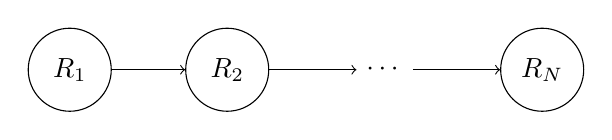
\begin{tikzpicture}[cnode/.style={draw,circle,minimum size=3em,inner sep=3pt}]
    \node[cnode] (1) at (0,0) {$R_1$};
    \node[cnode] (2) at (2, 0)  {$R_2$};
    \node (t) at (4, 0) {$\cdots$};
    \node[cnode] (n) at (6, 0)  {$R_N$};

    \draw[->] (1) edge (2) ;
    \draw[->] (2) edge (t) ;
    \draw[->] (t) edge (n) ;
\end{tikzpicture}
\caption{\em A random process $R$ for generating sequences of random length $N$. The arrows indicate transitions from one stage in the sequence to the next.}
\label{fig:R-process}
\end{figure}

We assume that each $R_t$ randomly takes some discrete or continuous value $r_t\in{\cal R}$,
and hence the probability (or probability density) of observing a particular
sequence $\vr$ of length $n=|\vr|$ is given by
\begin{eqnarray}
   p(\vec{R}\!=\!\vr) & = & p(N=n)\,p(R_1\!=\!r_1,\ldots,R_n\!=\!r_n\,|\,N=n)\,.
\end{eqnarray}
In practice, this definition presupposes that we know we have observed a {\em complete} sequence that started
at stage 1 and ended at stage $n$.
Suppose instead that the sequence $\vr$ was observed one stage at a time. How do we know if the
underlying process has actually terminated, or will instead
continue to generate another observed value $r_{n+1}$? 
Similarly, how do we know that the first observed value $r_1$ was not in fact
part of a longer, unobserved sequence of values?
We assume that the random process $R$ only ever produces complete sequences,
independently of the observation process, which might provide partial or complete sequences of values.
Furthermore, if the random process does not signal the start and end of generated sequences,
then an observed sequence might actually comprise multiple, contiguously generated subsequences.

In order to handle such difficulties, we consider any arbitrary sequence $\vr$ by default to be {\em incomplete},
and explicitly denote the corresponding, complete sequence by $\langle\vr\,\rangle$.
We can now introduce the notion of {\em partially complete} sequences. Thus, a {\em start sequence} is a generated sequence with an observed (or definite) start (at stage 1) 
but an unobserved (or indefinite) end, i.e.\ it might or might not terminate at stage $n$. This is denoted by $\langle\vr$ if we are truly uncertain as to the termination,
or by  $\langle\vr\,]$ if we actually know that the generated sequence does not terminate at stage $n$.
Similarly, an {\em end sequence} is a generated sequence with an observed end (at stage $n$) but an unobserved start, i.e.\ it might or might not have initiated at 
the observed stage 1. This is denoted by $\vr\,\rangle$ if we are truly uncertain as to sequence initiation,
or by  $[\vr\,\rangle$ if we actually know that the generated sequence was not initiated at stage $1$.
Clearly, we may also specify the remaining incomplete sequences, namely $[\vr\,]$, $\vr\,]$ and $[\vr$.

Under this augmented notation, knowledge about the start of a sequence can be encapsulated in 
a random indicator variable $\iota_{t-1}$, which takes on the value 1 if some observed $r_{t}$ is definitely the first stage in the
generated sequence, or the value 0 if it is not. Similarly, the random indicator variable $\tau_{t+1}$
takes on the value 1 if $r_{t}$ is definitely the last stage in the generated sequence, or the value 0 if it is not.
In general, these indicators allow us to handle the observation of possibly concatenated, multiple, generated sequences.
From now on, however, we shall assume (unless otherwise stated) that we are dealing with a single, contiguous sequence.
Thus, notionally, the indicators $\iota_0$ and $\tau_{n+1}$ can be thought to correspond to pseudo-stages 0 and $n+1$, such that
an arbitrary generated sequence is initiated at stage 0 and terminated at some random stage $N+1$.
This augmented random process is depicted in Figure~\ref{fig:random-process}. 
\begin{figure}[hbt]
\centering
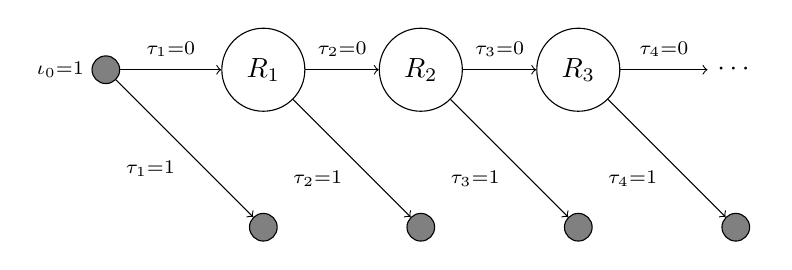
\begin{tikzpicture}[cnode/.style={draw,circle,minimum size=3em,inner sep=3pt}, onode/.style={fill=black!50, draw,circle,minimum size=1em}]
    \node (0i) at (-1,0) [right] {$\stackrel{\iota_0=1}{}$};
    \node[onode] (0) at (0,0) {};
    \node[cnode] (1) at (2,0) {$R_1$};
    \node[onode] (1t) at (2,-2) {};
    \node[cnode] (2) at (4, 0)  {$R_2$};
    \node[onode] (2t) at (4,-2) {};
    \node[cnode] (3) at (6, 0)  {$R_3$};
    \node[onode] (3t) at (6,-2) {};
    \node (t) at (8, 0) {$\cdots$};
    \node[onode] (tt) at (8, -2) {};

    \draw[->] (0) edge node [pos=0.5, above] {$\stackrel{\tau_1=0}{}$}  (1) ;
    \draw[->] (0) edge node [pos=0.5, below left] {$\stackrel{\tau_1=1}{}$} (1t) ;
    \draw[->] (1) edge node [pos=0.5, above] {$\stackrel{\tau_2=0}{}$}  (2) ;
    \draw[->] (1) edge node [pos=0.5, below left] {$\stackrel{\tau_2=1}{}$} (2t) ;
    \draw[->] (2) edge node [pos=0.5, above] {$\stackrel{\tau_3=0}{}$}  (3) ;
    \draw[->] (2) edge node [pos=0.5, below left] {$\stackrel{\tau_3=1}{}$} (3t) ;
    \draw[->] (3) edge node [pos=0.5, above] {$\stackrel{\tau_4=0}{}$}  (t) ;
    \draw[->] (3) edge node [pos=0.5, below left] {$\stackrel{\tau_4=1}{}$} (tt) ;
\end{tikzpicture}
\caption{\em A random process for generating complete sequences of random length,
with explicit stages for sequence initiation and termination. Multiple arrows exiting from a node indicate
different possible (mutually exclusive) stage transition pathways.}
\label{fig:random-process}
\end{figure}

The probability of a given complete sequence $\langle\vr\,\rangle$ is now defined as
\begin{eqnarray}
   p(\langle\vr\,\rangle)
& = & p(\iota_0\!=\!1,\tau_1\!=\!0,R_1=r_1,\tau_2\!=\!0,\ldots,\tau_n\!=\!0,R_n=r_n,\tau_{n+1}\!=\!1)
\label{eq:p_r_complete}
\,,
\end{eqnarray}
such that 
\begin{eqnarray}
   p(N\!=\!n) & = &  p(\iota_0\!=\!1,\tau_1\!=\!0,\ldots,\tau_n\!=\!0,\tau_{n+1}\!=\!1)\,.
\end{eqnarray}
This has the form of a generalised Bernoulli sequence.

Note that when the context is clear, we may for convenience drop explicit mention of the random variable $R_t$.
Similarly, we may denote $\iota_t=1$ by $\iota^+_t$, on the understanding that $\iota^-_t$ denotes the negation $\iota_t=0$.
Likewise, we may denote $\tau_t=1$ by $\tau^+_t$ and $\tau_t=0$ by $\tm_t$.
Hence, it is plausible to simplify equation~\eqref{eq:p_r_complete} as
\begin{eqnarray}
p(\langle\vr\,\rangle) 
& = & p(\iota_0^+,\tm_1,r_1,\ldots,\tm_n,r_n,\tau^+_{n+1})\,.
\end{eqnarray}
Consequently, we may simplify the explicitly terminated process of Figure~\ref{fig:random-process} 
to more resemble the implicitly terminatel process of Figure~\ref{fig:R-process}; the result is shown in Figure~\ref{fig:simple-random-process}.
\begin{figure}[hbt]
\centering
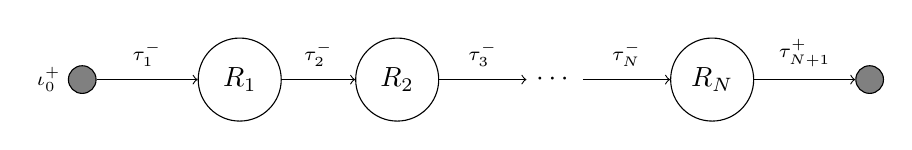
\begin{tikzpicture}[cnode/.style={draw,circle,minimum size=3em,inner sep=3pt}, onode/.style={fill=black!50, draw,circle,minimum size=1em}]
    \node (0i) at (-0.7,0) [right] {$\stackrel{\iota_0^+}{}$};
    \node[onode] (0) at (0,0) {};
    \node[cnode] (1) at (2,0) {$R_1$};
    \node[cnode] (2) at (4, 0)  {$R_2$};
    \node (t) at (6, 0) {$\cdots$};
    \node[cnode] (3) at (8, 0)  {$R_N$};
    \node[onode] (tt) at (10, 0) {};

    \draw[->] (0) edge node [pos=0.5, above] {$\stackrel{\tm_1}{}$}  (1) ;
    \draw[->] (1) edge node [pos=0.5, above] {$\stackrel{\tm_2}{}$}  (2) ;
    \draw[->] (2) edge node [pos=0.5, above] {$\stackrel{\tm_3}{}$}  (t) ;
    \draw[->] (t) edge node [pos=0.5, above] {$\stackrel{\tm_N}{}$}  (3) ;
    \draw[->] (3) edge node [pos=0.5, above] {$\stackrel{\tau^+_{N+1}}{}$} (tt) ;
\end{tikzpicture}
\caption{\em A simplified represenation of a random process for generating complete sequences of random length $N$,
with explicit stages for sequence initiation and termination, and explicit labelling of non-terminating transitions.}
\label{fig:simple-random-process}
\end{figure}

We can now handle both complete and partial sequences by introducing observed indicators $\ui$ and $\ut$
to correspond to the start-of-sequence and end-of-sequence symbols, respectively.
In particular, $\ui=1$ corresponds to `$\langle$' and $\ui=0$ corresponds to `$[$'; when the start of the sequence is unknown,
we let $\ui=*$ (see Section~\ref{sec:missing-values}). Likewise, $\ut=1$ corresponds to `$\rangle$', $\ut=0$ corresponds to `$]$', and
$\ut=*$ corresponds to unknown sequence termination.
Hence, in general, we write
\begin{eqnarray}
p(\ui,\vr,\ut)
& = & p(\iota_0\!=\!\ui,\tau_1\!=\!0,R_1\!=\!r_1,\ldots,\tau_n\!=\!0,R_n\!=\!r_n,\tau_{n+1}\!=\!\ut)
\nonumber\\
& = & p(\ui,\tm_1,r_1,\ldots,\tm_n,r_n,\ut)\,.
\label{eq:pr:gen}
\end{eqnarray}

\subsection{Missing Values}\label{sec:missing-values}

The main difference between a complete, generated sequence $\vr=(r_1,\ldots,r_n)$
and the observed sequence of values, say\footnote{We are ignoring the very real problem
of aligning the observed values with the generated stages. This difficulty can be partially alleviated under the assumption of stationary distributions, such that each stage behaves
like the previous one.} 
$\uvr=(\ur_1,\ldots,\ur_n)$, 
is the possibility that some values were unobserved, i.e.\ arbitrarily {\em missing} or systematically {\em hidden}.
For convenience, let $\ur_t=*$ denote the case where the  observed value of the $t$-th stage is missing,
just like $\ui=*$ or $\ut=*$ if we do not kow whether or not we observed the start or end of the generated sequence,
respectively.
The `*' symbol is just a representational device -- its presence has no effect on the computed probabilities, other than to indicate that any associated variable should be marginalised out. Thus, for example:
\begin{eqnarray}
p(\vr) 
& = & p(*,\tm_1,r_1,\ldots,\tm_n,r_n,*)~=~p(\tm_1,r_1,\ldots,\tm_n,r_n)\,.
\end{eqnarray}
In practice, we allow for both observed values and missing values by introducing an indicator function $\delta(\cdot)$,
where $\delta(x\!=\!y)=1$ if $x=y$ and $\delta(x\!=\!y)=0$ if $x\ne y$;  by definition, we take $\delta(x\!=\!*)=1$.
Hence, we obtain
\begin{eqnarray}
p(\ui,\vr,\ut) 
& = & 
\sum_{\iota_0=0}^{1}\delta(\iota_0\!=\!\ui)
\,\sum_{\tau_{n+1}=0}^{1}\delta(\tau_{n+1}\!=\!\ut)\;
p(\iota_0,\tm_1,r_1,\ldots,\tm_n,r_n,\tau_{n+1})\,.
\end{eqnarray}
In general, if the domain ${\cal R}$  is discrete, then the likelihood of an observed sequence is given by
\begin{eqnarray}
p(\ui,\uvr,\ut) 
& = & 
\sum_{\iota_0=0}^{1}\delta(\iota_0\!=\!\ui)
\,\sum_{\tau_{n+1}=0}^{1}\delta(\tau_{n+1}\!=\!\ut)
\sum_{r_1\in{\cal R}} \delta(r_1\!=\!\ur_1)
\cdots\sum_{r_n\in{\cal R}} \delta(r_n\!=\!\ur_n)
\nonumber\\
&& \hspace*{5mm}
p(\iota_0,\tm_1,r_1,\ldots,\tm_n,r_n,\tau_{n+1})\,.
\label{eq:pr:discrete}
\end{eqnarray}
Alternatively, if ${\cal R}$ is continuous, then the likelihood becomes
\begin{eqnarray}
p(\ui,\uvr,\ut) 
& = & 
\sum_{\iota_0=0}^{1}\delta(\iota_0\!=\!\ui)
\,\sum_{\tau_{n+1}=0}^{1}\delta(\tau_{n+1}\!=\!\ut)
\int_{{\cal R}} \delta(r_1\!-\!\ur_1)
\cdots\int_{{\cal R}} \delta(r_n\!-\!\ur_n)
\nonumber\\
&& \hspace*{5mm}
p(\iota_0,\tm_1,r_1,\ldots,\tm_n,r_n,\tau_{n+1})
\;dr_1\,dr_2\cdots dr_n
\,,
\end{eqnarray}
where $\delta(\cdot)$ is now the Dirac delta function, and where, by extension, we define $\delta(x\!-\!*)=1$.
On the understanding that $\sum$ and $\delta(x\!=\!y)$ must be swapped respectively for $\int$ and $\delta(x\!-\!y)$ as needed for a continuous 
or semi-continuous domain, we may henceforth simply utilise the discrete form~\eqref{eq:pr:discrete} without loss of generality.

\subsection{Generic Forward--Backward Algorithm}
\label{sec:forward-backward-basic}

The likelihood~\eqref{eq:pr:discrete} of an observed sequence $\uvr$ has been written in a computationally inefficient form,
but can in practice be efficiently evaluated by nesting the summations, using a modification of the {\em forward--backward algorithm} to include knowledge of
sequence initiation and termination.
The precise details of these calculations depend upon the chosen factorisation of the probability model, which is itself a function of
the explicit dependencies between various stages in the sequence. Such dependency modelling is dealt with further in Section~\ref{sec:markov-processes}.

Despite not knowing these dependencies in advance, however, the basic form of the forward--backward algorithm can still be formulated.
The first requirement is that the sequence process be {\em causal}, meaning that each stage of a sequence
%(including the termination stage but excluding the initiation stage)
 depends only on preceding stages, and never on future stages.
This causality allows us to split a generated sequence into two parts at some arbitrary {\em pivot} stage $t$, as shown in Figure~\ref{fig:forwar-backard}. The second requirement is that the dependence on past stages can be limited
in scope to some arbitrary {\em historical} stage $s$, as also shown.
\begin{figure}[hbt]
\centering
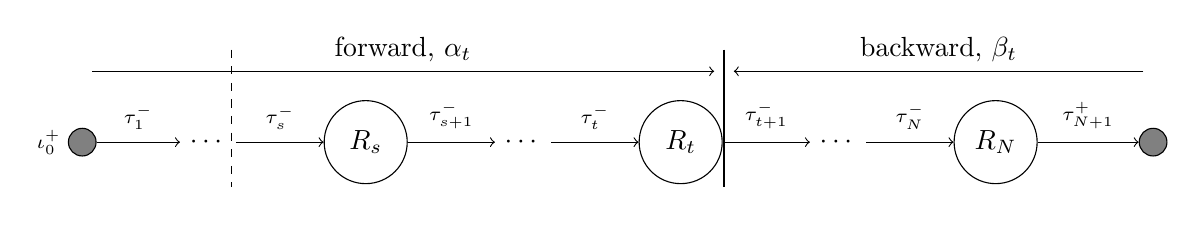
\begin{tikzpicture}[cnode/.style={draw,circle,minimum size=3em,inner sep=3pt}, onode/.style={fill=black!50, draw,circle,minimum size=1em}]
    \node (iota) at (-0.3, 0) [right] {$\stackrel{\iota_0^+}{}$};
    \node (0up) at (0.4, 0.9) {};
    \node[onode] (0) at (0.4, 0) {};
    \node (dots1) at (2, 0) {$\cdots$};
    \node (sup2) at (2.3, 1.3) {};
    \node (sdown) at (2.3, -0.7) {};
    \node[cnode] (s) at (4, 0) {$R_s$};
    \node (dots2) at (6, 0) {$\cdots$};
    \node (tup) at (8.55, 0.9) {};
    \node (tup2) at (8.55, 1.3) {};
    \node (tdown) at (8.55, -0.7) {};
    \node[cnode] (t) at (8, 0)  {$R_t$};
    \node (dots3) at (10, 0) {$\cdots$};
    \node[cnode] (N) at (12, 0)  {$R_N$};
    \node (Np1up) at (14, 0.9) {};
    \node[onode] (Np1) at (14, 0) {};

    \draw[->] (0) edge node [pos=0.5, above] {$\stackrel{\tm_1}{}$}  (dots1) ;
    \draw[->] (dots1) edge node [pos=0.5, above] {$\stackrel{\tm_s}{}$}  (s) ;
    \draw[->] (s) edge node [pos=0.5, above] {$\stackrel{\tm_{s+1}}{}$}  (dots2) ;
    \draw[->] (dots2) edge node [pos=0.5, above] {$\stackrel{\tm_t}{}$}  (t) ;
    \draw[->] (t) edge node [pos=0.5, above] {$\stackrel{\tm_{t+1}}{}$}  (dots3) ;
    \draw[->] (dots3) edge node [pos=0.5, above] {$\stackrel{\tm_{N}}{}$} (N) ;
    \draw[->] (N) edge node [pos=0.5, above] {$\stackrel{\tau^+_{N+1}}{}$} (Np1) ;

    \draw[dashed] (sup2) edge node {} (sdown) ;
    \draw[->] (0up) edge node [pos=0.5, above] {forward, $\alpha_t$} (tup) ;
    \draw[->] (Np1up) edge node [pos=0.5, above] {backward, $\beta_t$} (tup) ;
    \draw[-] (tup2) edge node {} (tdown) ;

\end{tikzpicture}
\caption{\em Causality allows the sequence to be partitioned at some pivot stage $t$, thereby dividing the sequence into past and future stages. Further
limitation of past dependencies to some historical stage $s$ defines the active window for
one step of the forward--backward algorithm.}
\label{fig:forwar-backard}
\end{figure}

Let us now define the sub-sequence $\vr_{s,t}=(r_s,r_{s+1},\ldots,r_t)$; by definition,
$\vr_{s,t}=(\,)$ if $s>t$. Furthermore, define the concatenation operator `$\circ$', such that
$\vr_{s,k}\circ\vr_{k+1,t}=\vr_{s,t}$.
Then observe, for a sufficiently long sequence (defined in Section~\ref{sec:markov-processes}), that
\begin{eqnarray}
p(\ui,\uvr,\ut) 
& = &
p(\ui,\uvr_{1,s-1}\circ\uvr_{s,t}\circ\uvr_{t+1,n},\ut)
\nonumber\\
& = &
\sum_{r_s\in{\cal R}} \delta(r_s\!=\!\ur_s)
\cdots\sum_{r_t\in{\cal R}} \delta(r_t\!=\!\ur_t)
\,p(\ui,\uvr_{1,s-1}\circ\vr_{s,t}\circ\uvr_{t+1,n},\ut)
\nonumber\\
& = &
\sum_{r_s\in{\cal R}} \delta(r_s\!=\!\ur_s)
\cdots\sum_{r_t\in{\cal R}} \delta(r_t\!=\!\ur_t)
\,p(\ui,\uvr_{1,s-1}\circ\vr_{s,t})
\,p(\uvr_{t+1,n},\ut\,|\,\ui,\uvr_{1,s-1}\circ\vr_{s,t})
\nonumber\\
& = &
\sum_{r_s\in{\cal R}} \delta(r_s\!=\!\ur_s)
\cdots\sum_{r_t\in{\cal R}} \delta(r_t\!=\!\ur_t)
\,\alpha_t(\vr_{s,t})\,\beta_t(\vr_{s,t})\,,
\end{eqnarray}
where
\begin{eqnarray}
\alpha_t(\vr_{s,t}) & = & p(\ui,\uvr_{1,s-1}\circ\vr_{s,t})~=~p(\ui,\tau_1^-,\ur_1,\ldots,\tm_{s-1},\ur_{s-1},
\tm_s,r_s,\ldots,\tm_t,r_t)
\label{eq:fwd-pass-basic}
\end{eqnarray}
is the foward factor,
and
\begin{eqnarray}
\beta_t(\vr_{s,t}) & = & p(\uvr_{t+1,n},\ut\,|\,\ui,\uvr_{1,s-1}\circ\vr_{s,t})
\nonumber\\& = &
p(\tm_{t+1},\ur_{t+1},\ldots,\tm_n,\ur_n,\ut\,|\,\ui,\tau_1^-,\ur_1,\ldots,\tm_{s-1},\ur_{s-1},
\tm_s,r_s,\ldots,\tm_t,r_t)\
\label{eq:bwd-pass-basic}
\end{eqnarray}
is the backward factor.
The entire forward pass of the forward--backward algorithm starts from some initial, historical stage $t_0$ and
progressively computes $\alpha_t$ forward along the sequence for each applicable stage $t_0\le t\le n$. Likewise,
the backward pass starts at termination stage, and computes $\beta_t$
backwards along the sequence for each applicable stage $t_0\le t\le n$. The precise details of these calculations rely upon
the nature of the fine-grained dependencies, as disdcussed in the next section.

%%%%%%%%%%%%%%%%%%%%%%%%%%%%%%%%%%%
\section{Markov Sequence Processes}
\label{sec:markov-processes}
In Section~\ref{sec:random-processes}, we defined a causal random sequence process $R$, such that each stage of a sequence,
including the termination stage, depends only on the preceding stages.
This causal process, depicted in Figure~\ref{fig:causal-process}, is simply the random process from
Figure~\ref{fig:simple-random-process} with additional, explicit dependencies (in the form of dashed arrows).
\begin{figure}[hbt]
\centering
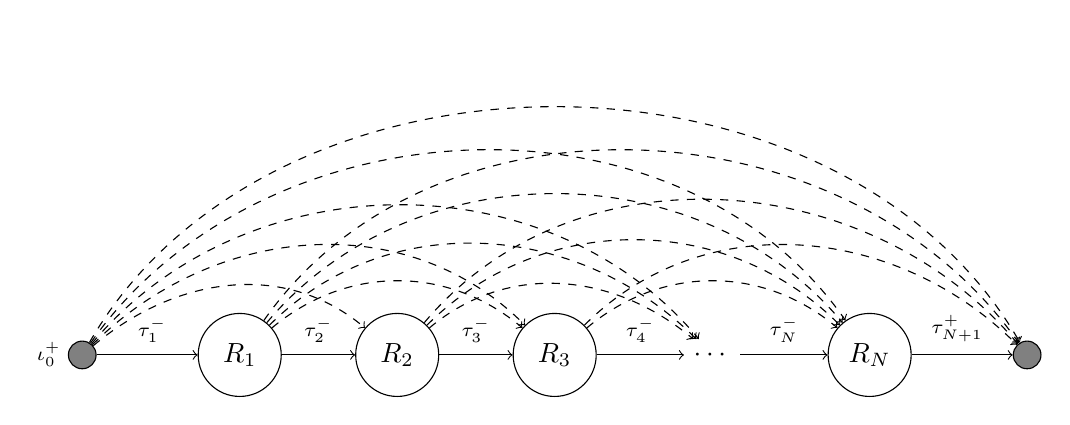
\begin{tikzpicture}[cnode/.style={draw,circle,minimum size=3em,inner sep=3pt}, onode/.style={fill=black!50, draw,circle,minimum size=1em}]
    \node (0i) at (-0.7,0) [right] {$\stackrel{\iota_0^+}{}$};
    \node[onode] (0) at (0,0) {};
    \node[cnode] (1) at (2,0) {$R_1$};
    \node[cnode] (2) at (4, 0)  {$R_2$};
    \node[cnode] (3) at (6, 0)  {$R_3$};
    \node (t) at (8, 0) {$\cdots$};
    \node[cnode] (N) at (10, 0)  {$R_N$};
    \node[onode] (tt) at (12, 0) {};

    \draw[->] (0) edge node [pos=0.55, above] {$\stackrel{\tm_1}{}$}  (1) ;
    \draw[->] (1) edge node [pos=0.5, above] {$\stackrel{\tm_2}{}$}  (2) ;
    \draw[->] (2) edge node [pos=0.5, above] {$\stackrel{\tm_3}{}$}  (3) ;
    \draw[->] (3) edge node [pos=0.5, above] {$\stackrel{\tm_4}{}$}  (t) ;
    \draw[->] (t) edge node [pos=0.5, above] {$\stackrel{\tm_N}{}$}  (N) ;
    \draw[->] (N) edge node [pos=0.45, above] {$\stackrel{\tau^+_{N+1}}{}$} (tt) ;

   \begin{scope}[dashed]
    \draw[->] (0) to[out=40,in=140] (2) ;
    \draw[->] (0) to[out=45,in=135] (3) ;
    \draw[->] (0) to[out=50,in=130] (t) ;
    \draw[->] (0) to[out=55,in=125] (N) ;
    \draw[->] (0) to[out=60,in=120] (tt) ;
    \draw[->] (1) to[out=40,in=140] (3) ;
    \draw[->] (1) to[out=45,in=135] (t) ;
    \draw[->] (1) to[out=50,in=130] (N) ;
    \draw[->] (1) to[out=55,in=125] (tt) ;
    \draw[->] (2) to[out=40,in=140] (t) ;
    \draw[->] (2) to[out=45,in=135] (N) ;
    \draw[->] (2) to[out=50,in=130] (tt) ;
    \draw[->] (3) to[out=40,in=140] (N) ;
    \draw[->] (3) to[out=45,in=135] (tt) ;
   \end{scope}
\end{tikzpicture}
\caption{\em A fully-dependent, causal process for generating complete, random sequences of random length $N$.
Solid arrows indicate stage transitions. 
Both dashed arrows and solid arrows indicate parent--child dependencies, such that each stage is conditionally dependent on the preceding stages.}
\label{fig:causal-process}
\end{figure}
Hence, under the Markov assumption of conditional independence,
the causal sequence process leads to the fully-dependent conditional model
\begin{eqnarray}
p(\iota_0,\vr,\tau_{n+1}) & = &
p(\iota_0,\tm_1,r_1,\tm_2,r_2,\ldots,\tm_n,r_n,\tau_{n+1})
\nonumber\\
& = &
p(\iota_0)
\,p(\tm_1\,|\,\iota_0)
\,p(r_1\,|\,\iota_0,\tm_1)
\,p(\tm_2\,|\,\iota_0,\tm_1,r_1)
\, p(r_2\,|\,\iota_0,\tm_1,r_1,\tm_2)
\nonumber\\
&&
\cdots
p(\tm_n\,|\,\iota_0,\ldots,\tm_{n-1},r_{n-1})
p(r_n\,|\,\iota_0,\ldots,\tm_{n})
\, p(\tau_{n+1}\,|\,\iota_0,\ldots,r_n)
\nonumber\\
& = &
p(\iota_0)
\left\{\prod_{t=1}^{n}p(\tm_t,r_t\,|\,\iota_0,\vec{\tau}^-_{1,t-1},\vr_{1,t-1})\right\}
 p(\tau_{n+1}\,|\,\iota_0,\vec{\tau}^-_{1,n},\vr_{1,n})
\,.
\label{eq:temporal-model-full}
\end{eqnarray}

In practice, this fully-dependent model is considerably simplified by dropping some or even most of the explicit (dashed) dependencies.
For example, one might limit the 
conditionality on past stages to a maximum of $m$ depenencies.
This leads to the so-called {\em $m$-th order Markov model},
shown in Figure~\ref{fig:markov-m}.
\begin{figure}[hbt]
\centering
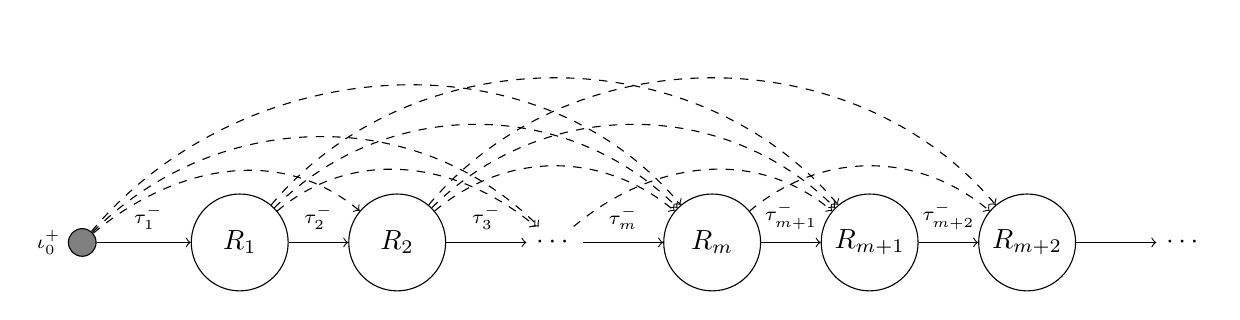
\begin{tikzpicture}[cnode/.style={draw,circle,minimum size=3.5em,inner sep=3pt}, onode/.style={fill=black!50, draw,circle,minimum size=1em}]
    \node (0i) at (-0.7,0) [right] {$\stackrel{\iota_0^+}{}$};
    \node[onode] (0) at (0,0) {};
    \node[cnode] (1) at (2,0) {$R_1$};
    \node[cnode] (2) at (4, 0)  {$R_2$};
    \node (t) at (6, 0) {$\cdots$};
    \node[cnode] (m) at (8, 0)  {$R_m$};
    \node[cnode] (mp1) at (10, 0)  {$R_{m+1}$};
    \node[cnode] (mp2) at (12, 0)  {$R_{m+2}$};
    \node (t2) at (14, 0) {$\cdots$};

    \draw[->] (0) edge node [pos=0.55, above] {$\stackrel{\tm_1}{}$}  (1) ;
    \draw[->] (1) edge node [pos=0.5, above] {$\stackrel{\tm_2}{}$}  (2) ;
    \draw[->] (2) edge node [pos=0.5, above] {$\stackrel{\tm_3}{}$}  (t) ;
    \draw[->] (t) edge node [pos=0.5, above] {$\stackrel{\tm_m}{}$}  (m) ;
    \draw[->] (m) edge node [pos=0.5, above] {$\stackrel{\tm_{m+1}}{}$}  (mp1) ;
    \draw[->] (mp1) edge node [pos=0.5, above] {$\stackrel{\tm_{m+2}}{}$}  (mp2) ;
    \draw[->] (mp2) edge node [pos=0.5, above] {}  (t2) ;

   \begin{scope}[dashed]
    \draw[->] (0) to[out=40,in=140] (2) ;
    \draw[->] (0) to[out=45,in=135] (t) ;
    \draw[->] (0) to[out=50,in=130] (m) ;
    \draw[->] (1) to[out=40,in=140] (t) ;
    \draw[->] (1) to[out=45,in=135] (m) ;
    \draw[->] (1) to[out=50,in=130] (mp1) ;
    \draw[->] (2) to[out=40,in=140] (m) ;
    \draw[->] (2) to[out=45,in=135] (mp1) ;
    \draw[->] (2) to[out=50,in=130] (mp2) ;
    \draw[->] (t) to[out=40,in=140] (mp1) ;
    \draw[->] (m) to[out=40,in=140] (mp2) ;
   \end{scope}
\end{tikzpicture}
\caption{\em An $m$-th order Markov sequence process of arbitrary length (here $n\ge m+2$).}
\label{fig:markov-m}
\end{figure}
The corresponding likelihood model is given by
\begin{eqnarray}
p(\iota_0,\vr,\tau_{n+1}) & = &
p(\iota_0)
\left\{\prod_{t=1}^{m}p(\tm_t,r_t\,|\,\iota_0,\vec{\tau}^-_{1,t-1},\vr_{1,t-1})\right\}
\nonumber\\&&
\left\{\prod_{t=m+1}^{n}p(\tm_t,r_t\,|\,\vec{\tau}^-_{t-m,t-1},\vr_{t-m,t-1})\right\}
p(\tau_{n+1}\,|\,\vec{\tau}^-_{n-m+1,n},\vr_{n-m+1,n})\,,
\label{eq:mth-order}
\end{eqnarray}
for $n\ge m$.

An example from the realm of natural language understanding is the lexicographical analysis of the character
sequences of words using bigrams (pairs of adjacent characters, corresponding to $m=1$), and trigrams 
(triples of adjacent characters, corresponding to $m=2$), etc.
The second-order Markov sequence process, for example, is depicted in Figure~\ref{fig:causal-process-2}.
\begin{figure}[hbt]
\centering
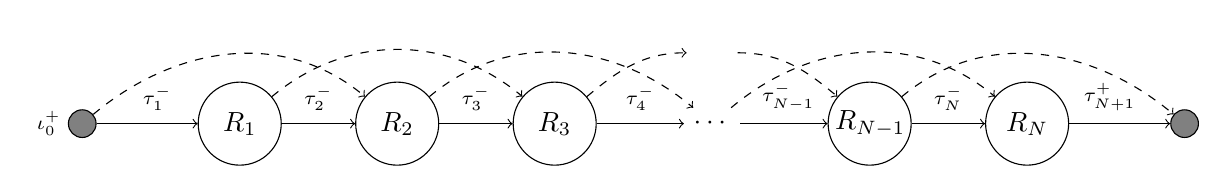
\begin{tikzpicture}[cnode/.style={draw,circle,minimum size=3em,inner sep=3pt}, onode/.style={fill=black!50, draw,circle,minimum size=1em}]
    \node (0i) at (-0.7,0) [right] {$\stackrel{\iota_0^+}{}$};
    \node[onode] (0) at (0,0) {};
    \node[cnode] (1) at (2,0) {$R_1$};
    \node[cnode] (2) at (4, 0)  {$R_2$};
    \node[cnode] (3) at (6, 0)  {$R_3$};
    \node (td) at (7.8,0.9) {};
    \node (t) at (8, 0) {$\cdots$};
    \node (Nm1d) at (8.2,0.9) {};
    \node[cnode] (Nm1) at (10, 0)  {\begin{varwidth}{1.5em}$\!\!\!R_{N-1}$\end{varwidth}};
    \node[cnode] (N) at (12, 0)  {$R_N$};
    \node[onode] (tt) at (14, 0) {};

    \draw[->] (0) edge node [pos=0.6, above] {$\stackrel{\tm_1}{}$}  (1) ;
    \draw[->] (1) edge node [pos=0.5, above] {$\stackrel{\tm_2}{}$}  (2) ;
    \draw[->] (2) edge node [pos=0.5, above] {$\stackrel{\tm_3}{}$}  (3) ;
    \draw[->] (3) edge node [pos=0.5, above] {$\stackrel{\tm_4}{}$}  (t) ;
    \draw[->] (t) edge node [pos=0.55, above] {$\stackrel{\tm_{N-1}}{}$}  (Nm1) ;
    \draw[->] (Nm1) edge node [pos=0.5, above] {$\stackrel{\tm_N}{}$}  (N) ;
    \draw[->] (N) edge node [pos=0.4, above] {$\stackrel{\tau^+_{N+1}}{}$}  (tt) ;

   \begin{scope}[dashed]
    \draw[->] (0) to[out=40,in=140] (2) ;
    \draw[->] (1) to[out=40,in=140] (3) ;
    \draw[->] (2) to[out=40,in=140] (t) ;
    \draw[->] (3) to[out=40,in=180] (td) ;
    \draw[->] (t) to[out=40,in=140] (N) ;
    \draw[->] (Nm1d) to[in=140,out=0] (Nm1) ;
    \draw[->] (Nm1) to[out=40,in=140] (tt) ;
   \end{scope}
\end{tikzpicture}
\caption{\em A second-order Markov sequence process of random length $N$.}
\label{fig:causal-process-2}
\end{figure}

In the special case of $m=1$, the first-order Markov model,
depicted in Figure~\ref{fig:simple-random-process}, takes on the especially-simple conditional form
 of
\begin{eqnarray}
p(\iota_0,\vr,\tau_{n+1}) & = &
p(\iota_0)\,p(\tm_1,r_1\,|\,\iota_0)
\left\{\prod_{t=2}^{n}p(\tm_t,r_t\,|\,\tm_{t-1},r_{t-1})\right\}
\,p(\tau_{n+1}\,|\,\tm_n,r_n)
\,,
\end{eqnarray}
for $n>0$.

\subsection{Markov Forward--Backward Algorithm}
\label{sec:forward-backward-markov}

The basic description of the generic forward--backward algorithm in Section~\ref{sec:forward-backward-basic}
can now be refined under the restriction of the causal sequence process to an $m$-th order Markov process.
Specifically, for any stage $1\le t\le n$, we take the limiting historical stage to be $s=\max(1, t-m+1)$.
Then, for a sufficiently long sequence (i.e.\ $n\ge m$), the forward factor~\eqref{eq:fwd-pass-basic} may be
computed for stages $t=m,m+1,\ldots,n$ via
%\begin{eqnarray}
%\alpha_t(\vr_{1,t}) & = & p(\iota_0,\tm_1,r_1,\ldots,\tm_t,r_t)
%~=~
%p(\iota_0)\,\prod_{i=1}^{t}p(\tm_i,r_i\,|\,\iota_0,\vec{\tau}^-_{1,i-1},\vr_{1,i-1})\,.
%\label{eq:fwd-pass-m-init}
%\end{eqnarray}
%Furthermore, if $t<m-1$ then at stage $t+1$ we have
%\begin{eqnarray}
%\alpha_{t+1}(\vr_{1,t+1}) & = & p(\iota_0,\tm_1,r_1,\ldots,\tm_{t+1},r_{t+1})
%~=~
%p(\iota_0)\,\prod_{i=1}^{t+1}p(\tm_i,r_i\,|\,\iota_0,\vec{\tau}^-_{1,i-1},\vr_{1,i-1})
%\nonumber\\& = &
%\alpha_t(\vr_{1,t})\,p(\tm_{t+1},r_{t+1}\,|\,\iota_0,\vec{\tau}^-_{1,t},\vr_{1,t})\,.
%\end{eqnarray}
%Note that for $m>1$ the forward pass commences from
%\begin{eqnarray}
%\alpha_1(r_1) & = &  p(\iota_0)\,p(\tm_1,r_1\,|\,\iota_0)\,.
%\end{eqnarray}
%However, if the sequence is sufficiently long, then for later stages $t\ge m$ we obtain
\begin{eqnarray}
\hspace*{-5mm}
\alpha_t(\vr_{t-m+1,t}) & = & p(\ui,\tm_1,\ur_1,\ldots,\tm_{t-m},\ur_{t-m},\tm_{t-m+1},r_{t-m+1},\ldots,\tm_t,r_t)
\nonumber\\& = &
\sum_{\iota_0=0}^{1}\delta(\iota_0\!=\!\ui)\,
\sum_{r_1\in{\cal R}} \delta(r_1\!=\!\ur_1)\,
\cdots
\sum_{r_{t-m}\in{\cal R}} \delta(r_{t-m}\!=\!\ur_{t-m})
\nonumber\\&&
p(\iota_0)\left\{\prod_{i=1}^{m}p(\tm_i,r_i\,|\,\iota_0,\vec{\tau}^-_{1,i-1},\vr_{1,i-1})\right\}
\left\{\prod_{i=m+1}^{t}p(\tm_i,r_i\,|\,\vec{\tau}^-_{i-m,i-1},\vr_{i-m,i-1})\right\}\,,
\label{eq:fwd-pass-m}
\end{eqnarray}
from equation~\eqref{eq:mth-order}. 
Furthermore, if $m\le t<n$ then we may simplify the forward pass by observing that
\begin{eqnarray}
\!\!\!\!\!\!\!
\alpha_{t+1}(\vr_{t-m+2,t+1}) & = & 
p(\ui,\tm_1,\ur_1,\ldots,\tm_{t-m+1},\ur_{t-m+1},\tm_{t-m+2},r_{t-m+2},\ldots,\tm_{t+1},r_{t+1})
\nonumber\\& = &
\sum_{\iota_0=0}^{1}\delta(\iota_0\!=\!\ui)\,
\sum_{r_1\in{\cal R}} \delta(r_1\!=\!\ur_1)\,
\cdots
\sum_{r_{t-m+1}\in{\cal R}} \delta(r_{t-m+1}\!=\!\ur_{t-m+1})
\nonumber\\&&
p(\iota_0)\left\{\prod_{i=1}^{m}p(\tm_i,r_i\,|\,\iota_0,\vec{\tau}^-_{1,i-1},\vr_{1,i-1})\right\}
\left\{\prod_{i=m+1}^{t+1}p(\tm_i,r_i\,|\,\vec{\tau}^-_{i-m,i-1},\vr_{i-m,i-1})\right\}
\nonumber\\& = &\!\!\!
\sum_{r_{t-m+1}\in{\cal R}} \delta(r_{t-m+1}\!=\!\ur_{t-m+1})\,\alpha_t(\vr_{t-m+1,t})
\,p(\tm_{t+1},r_{t+1}\,|\,\vec{\tau}^-_{t-m+1,t},\vr_{t-m+1,t})\,.
\label{eq:fwd-pass-m-recursive}
\end{eqnarray}
Effectively, this recursive relation comes from moving the size-$m$ active window from stage $t$ to stage $t+1$ and thereby marginalising over the
observation $\ur_{t-m+1}$ that has now left the window.
Note that for the special case of $m=1$, this forward pass reduces to
\begin{eqnarray}
\alpha_1(r_1) & = &  \sum_{\iota_0=0}^{1}\delta(\iota_0\!=\!\ui)\,
p(\iota_0)\,p(\tm_1,r_1\,|\,\iota_0)\,,
\nonumber\\
\alpha_{t}(r_{t}) & = &
\sum_{r_{t-1}\in{\cal R}} \delta(r_{t-1}\!=\!\ur_{t-1})\,\alpha_{t-1}(r_{t-1})
\,p(\tm_{t},r_{t}\,|\,\tm_{t-1},r_{t-1})
\hspace*{2mm}\mbox{ for $t=2,\ldots,n$}
\,.
\end{eqnarray}

Similarly, the backward pass is also well-defined for stages $t\ge m$, such that the backward factor~\eqref{eq:bwd-pass-basic} becomes
\begin{eqnarray}
\beta_t(\vr_{t-m+1,t}) & = & 
p(\tm_{t+1},\ur_{t+1},\ldots,\tm_n,\ur_n,\ut\,|\,\tm_{t-m+1},r_{t-m+1},\ldots,\tm_t,r_t)
\nonumber\\& = &
\sum_{r_{t+1}\in{\cal R}} \delta(r_{t+1}\!=\!\ur_{t+1})\,\cdots
\sum_{r_{n}\in{\cal R}} \delta(r_{n}\!=\!\ur_{n})\,
\sum_{\tau_{n+1}=0}^{1}\delta(\tau_{n+1}\!=\!\ut_{n+1})
\nonumber\\
&&{}
\left\{\prod_{i=t+1}^n
p(\tm_{i},r_{i}\,|\,\vec{\tau}^-_{i-m,i-1},\vr_{i-m,i-1})\right\}
p(\tau_{n+1}\,|\,\vec{\tau}^-_{n-m+1,n},\vr_{n-m+1,n})
\,.
\end{eqnarray}
Likewise, if $m<t\le n$ then we may move the window backwards from stage $t$ to stage $t-1$, thereby obtaining the recursive relation
\begin{eqnarray}
\beta_{t-1}(\vr_{t-m,t-1}) & = & 
p(\tm_{t},\ur_{t},\ldots,\tm_n,\ur_n,\ut\,|\,\tm_{t-m},r_{t-m},\ldots,\tm_{t-1},r_{t-1})
\nonumber\\& = &
\sum_{r_{t}\in{\cal R}} \delta(r_{t}\!=\!\ur_{t})\,\cdots
\sum_{r_{n}\in{\cal R}} \delta(r_{n}\!=\!\ur_{n})\,
\sum_{\tau_{n+1}=0}^{1}\delta(\tau_{n+1}\!=\!\ut_{n+1})
\nonumber\\
&&{}
\left\{\prod_{i=t}^n
p(\tm_{i},r_{i}\,|\,\vec{\tau}^-_{i-m,i-1},\vr_{i-m,i-1})\right\}
p(\tau_{n+1}\,|\,\vec{\tau}^-_{n-m+1,n},\vr_{n-m+1,n})
\nonumber\\& = &
\sum_{r_{t}\in{\cal R}} \delta(r_{t}\!=\!\ur_{t})\,
p(\tm_{t},r_{t}\,|\,\vec{\tau}^-_{t-m,t-1},\vr_{t-m,t-1})\,\beta_{t}(\vr_{t-m+1,t})
\,.
\end{eqnarray}
Effectively, moving the size-$m$ active window from stage $t$ to stage $t-1$ allows us to marginalise over the
observation $\ur_{t}$ that has now left the window.
For the special case of $m=1$, this backward pass reduces to
\begin{eqnarray}
\beta_n(r_n) & = &  \sum_{\tau_{n+1}=0}^{1}\delta(\tau_{n+1}\!=\!\ut)\,
p(\tau_{n+1}\,|\,\tm_n,r_n)\,,
\nonumber\\
\beta_{t}(r_{t}) & = &
\sum_{r_{t+1}\in{\cal R}} \delta(r_{t+1}\!=\!\ur_{t+1})\,
p(\tm_{t+1},r_{t+1}\,|\,\tm_{t},r_{t})
\,\beta_{t+1}(r_{t+1})\hspace*{2mm}\mbox{ for $t=n-1,\ldots,1$}
\,.
\end{eqnarray}
Note that for a short sequence of length $n<m$ we must evaluate the observation likelihood~\eqref{eq:pr:discrete} directly using
equation~\eqref{eq:mth-order}. The forward--backward algorithm is of no help in such a case, since the active window overlaps
both ends of the sequence, namely $\ui$ and $\ut$, making the dependencies highly stage specific.

%%%%%%%%%%%%%%%%%%%%%%%%%%%%%%%%%%%%%%%%%
\section{Stateful Markov Sequence Processes}
Consider the fully-dependent causal process $R$ depicted in Figure~\ref{fig:causal-process}.
Suppose now that the random variable $R_t$ at stage $t$ can be decomposed into the tuple
$R_t=(S_t,X_t)$, where $S_t$ is a random {\em state} variable taking values $s_t\in{\cal S}$, and $X_t$
is a random {\em value} variable taking values $x_t\in{\cal X}$.
We make the common presumption that the stage transitions in the sequence generating process are entirely between states, e.g.\ from $S_{t-1}$ to $S_t$.
It follows from causation that the value $x_t$ is generated after the state $s_t$ has been determined, i.e.\ $X_t$ depends upon $S_t$.
Consequently, the fully-dependent  stateful sequence process, shown in Figure~\ref{fig:stateful-full}, is derived from Figure~\ref{fig:causal-process}
by replacing each node $R_t$ by the pair of nodes $S_t$ and $X_t$ with a dependency from $S_t$ to $X_t$, such that every {\em afferent} dependency pointing to $R_t$ becomes two dependencies pointing to $S_t$ and $X_t$, and every {\em efferent} dependency pointing from $R_t$ becomes two dependencies pointing from $S_t$ and $X_t$, respectively.
\begin{figure}[hbt]
\centering
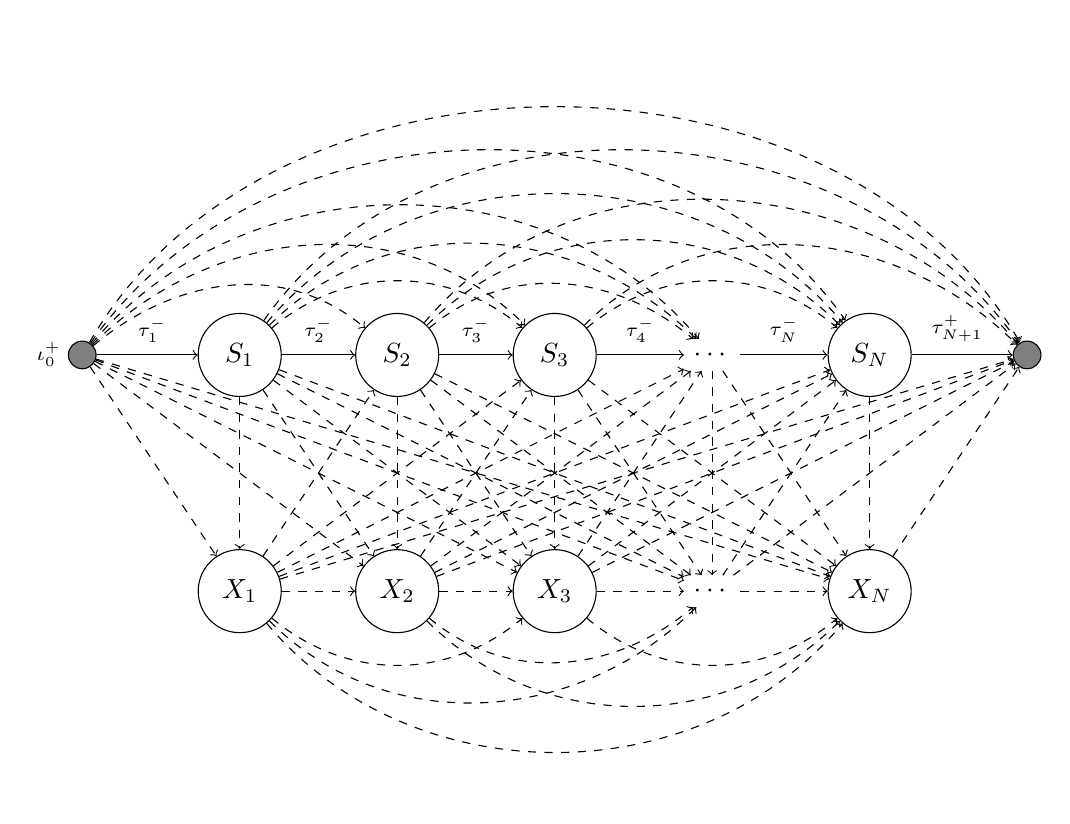
\begin{tikzpicture}[cnode/.style={draw,circle,minimum size=3em,inner sep=3pt}, onode/.style={fill=black!50, draw,circle,minimum size=1em}]
    \node (0i) at (-0.7,0) [right] {$\stackrel{\iota_0^+}{}$};
    \node[onode] (0) at (0,0) {};
    \node[cnode] (1) at (2,0) {$S_1$};
    \node[cnode] (1x) at (2,-3) {$X_1$};
    \node[cnode] (2) at (4, 0)  {$S_2$};
    \node[cnode] (2x) at (4, -3)  {$X_2$};
    \node[cnode] (3) at (6, 0)  {$S_3$};
    \node[cnode] (3x) at (6, -3)  {$X_3$};
    \node (t) at (8, 0) {$\cdots$};
    \node (tx) at (8, -3) {$\cdots$};
    \node[cnode] (N) at (10, 0)  {$S_N$};
    \node[cnode] (Nx) at (10, -3)  {$X_N$};
    \node[onode] (tt) at (12, 0) {};

    \draw[->] (0) edge node [pos=0.55, above] {$\stackrel{\tm_1}{}$}  (1) ;
    \draw[->] (1) edge node [pos=0.5, above] {$\stackrel{\tm_2}{}$}  (2) ;
    \draw[->] (2) edge node [pos=0.5, above] {$\stackrel{\tm_3}{}$}  (3) ;
    \draw[->] (3) edge node [pos=0.5, above] {$\stackrel{\tm_4}{}$}  (t) ;
    \draw[->] (t) edge node [pos=0.5, above] {$\stackrel{\tm_N}{}$}  (N) ;
    \draw[->] (N) edge node [pos=0.45, above] {$\stackrel{\tau^+_{N+1}}{}$} (tt) ;

   \begin{scope}[dashed]
    \draw[->] (0) to[out=40,in=140] (2) ;
    \draw[->] (0) to[out=45,in=135] (3) ;
    \draw[->] (0) to[out=50,in=130] (t) ;
    \draw[->] (0) to[out=55,in=125] (N) ;
    \draw[->] (0) to[out=60,in=120] (tt) ;
    \draw[->] (1) to[out=40,in=140] (3) ;
    \draw[->] (1) to[out=45,in=135] (t) ;
    \draw[->] (1) to[out=50,in=130] (N) ;
    \draw[->] (1) to[out=55,in=125] (tt) ;
    \draw[->] (2) to[out=40,in=140] (t) ;
    \draw[->] (2) to[out=45,in=135] (N) ;
    \draw[->] (2) to[out=50,in=130] (tt) ;
    \draw[->] (3) to[out=40,in=140] (N) ;
    \draw[->] (3) to[out=45,in=135] (tt) ;
   \end{scope}

   \begin{scope}[dashed]
    \draw[->] (0) to (1x) ;
    \draw[->] (0) to (2x) ;
    \draw[->] (0) to (3x) ;
    \draw[->] (0) to (tx) ;
    \draw[->] (0) to (Nx) ;

    \draw[->] (1) to (1x) ;
    \draw[->] (1) to (2x) ;
    \draw[->] (1) to (3x) ;
    \draw[->] (1) to (tx) ;
    \draw[->] (1) to (Nx) ;
    \draw[->] (2) to (2x) ;
    \draw[->] (2) to (3x) ;
    \draw[->] (2) to (tx) ;
    \draw[->] (2) to (Nx) ;
    \draw[->] (3) to (3x) ;
    \draw[->] (3) to (tx) ;
    \draw[->] (3) to (Nx) ;
    \draw[->] (t) to (tx) ;
    \draw[->] (t) to (Nx) ;
    \draw[->] (N) to (Nx) ;

    \draw[->] (1x) to (2) ;
    \draw[->] (1x) to (3) ;
    \draw[->] (1x) to (t) ;
    \draw[->] (1x) to (N) ;
    \draw[->] (2x) to (3) ;
    \draw[->] (2x) to (t) ;
    \draw[->] (2x) to (N) ;
    \draw[->] (3x) to (t) ;
    \draw[->] (3x) to (N) ;
    \draw[->] (tx) to (N) ;

    \draw[->] (1x) to (tt) ;
    \draw[->] (2x) to (tt) ;
    \draw[->] (3x) to (tt) ;
    \draw[->] (tx) to (tt) ;
    \draw[->] (Nx) to (tt) ;
   \end{scope}

   \begin{scope}[dashed]
    \draw[->] (1x) to (2x) ;
    \draw[->] (2x) to (3x) ;
    \draw[->] (3x) to (tx) ;
    \draw[->] (tx) to (Nx) ;

    \draw[->] (1x) to[out=-40,in=-140] (3x) ;
    \draw[->] (1x) to[out=-45,in=-135] (tx) ;
    \draw[->] (1x) to[out=-50,in=-130] (Nx) ;
    \draw[->] (2x) to[out=-40,in=-140] (tx) ;
    \draw[->] (2x) to[out=-45,in=-135] (Nx) ;
    \draw[->] (3x) to[out=-40,in=-140] (Nx) ;
   \end{scope}
\end{tikzpicture}
\caption{\em A fully-dependent, causal, stateful process for generating complete, random sequences of random length $N$, consisting of pairs of states and values.}
\label{fig:stateful-full}
\end{figure}
For convenience, we may notionally separate the states from the corresponding values at each stage by loosely defining
\begin{eqnarray}
\vr & = & (r_1,r_2,\ldots,r_n)
\nonumber\\& = & 
((s_1,x_1),(s_2,x_2),\ldots,(s_n,x_n))
\nonumber\\& \equiv & 
(s_1,\ldots,s_n)\odot (x_1,\ldots,x_n)~=~(\vs,\vx)\,.
\end{eqnarray}
Hence, the joint likelihood of a fully-dependent state--value sequence is now derived from model~\eqref{eq:temporal-model-full} as
\begin{eqnarray}
p(\iota_0,\vs,\vx,\tau_{n+1}) & = &
p(\iota_0,\tm_1,s_1,x_1,\tm_2,s_2,x_2,\ldots,\tm_n,s_n,x_n,\tau_{n+1})
\nonumber\\
& = &
p(\iota_0)
\left\{\prod_{t=1}^{n}p(\tm_t,s_t\,|\,\iota_0,\vec{\tau}^-_{1,t-1},\vs_{1,t-1},\vx_{1,t-1})\,p(x_t\,|\,\iota_0,\vec{\tau}^-_{1,t-1},\vs_{1,t},\vx_{1,t-1})\right\}
\nonumber\\&&{}\times
 p(\tau_{n+1}\,|\,\iota_0,\vec{\tau}^-_{1,n},\vs_{1,n},\vx_{1,n})
\,.
\label{eq:stateful-model-full}
\end{eqnarray}

In practice, the dependence of $S_t$ and $X_t$ on $X_{t-1}$ (and further historical values) induces a regression model of some complexity,
especially if the set ${\cal X}$ of values is continuous and/or multi-dimensional. Also, such a dependency causes difficulties handling missing values (see Section~\ref{sec:hidden-state}).
Lastly, as we discussed earlier, the general `spirit' of  stateful processes is that the state drives the value, not the other way around.
Hence, common practice is to limit the dependicies of $X_t$ to only  the current and previous states, as shown in Figure~\ref{fig:stateful-sub}.
\begin{figure}[hbt]
\centering
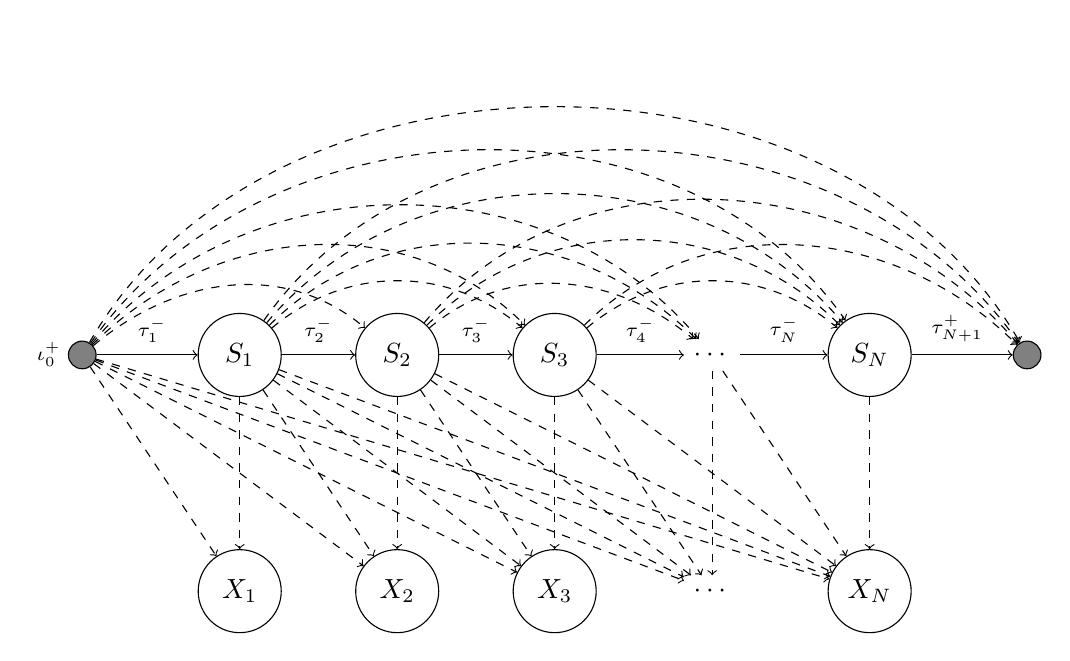
\begin{tikzpicture}[cnode/.style={draw,circle,minimum size=3em,inner sep=3pt}, onode/.style={fill=black!50, draw,circle,minimum size=1em}]
    \node (0i) at (-0.7,0) [right] {$\stackrel{\iota_0^+}{}$};
    \node[onode] (0) at (0,0) {};
    \node[cnode] (1) at (2,0) {$S_1$};
    \node[cnode] (1x) at (2,-3) {$X_1$};
    \node[cnode] (2) at (4, 0)  {$S_2$};
    \node[cnode] (2x) at (4, -3)  {$X_2$};
    \node[cnode] (3) at (6, 0)  {$S_3$};
    \node[cnode] (3x) at (6, -3)  {$X_3$};
    \node (t) at (8, 0) {$\cdots$};
    \node (tx) at (8, -3) {$\cdots$};
    \node[cnode] (N) at (10, 0)  {$S_N$};
    \node[cnode] (Nx) at (10, -3)  {$X_N$};
    \node[onode] (tt) at (12, 0) {};

    \draw[->] (0) edge node [pos=0.55, above] {$\stackrel{\tm_1}{}$}  (1) ;
    \draw[->] (1) edge node [pos=0.5, above] {$\stackrel{\tm_2}{}$}  (2) ;
    \draw[->] (2) edge node [pos=0.5, above] {$\stackrel{\tm_3}{}$}  (3) ;
    \draw[->] (3) edge node [pos=0.5, above] {$\stackrel{\tm_4}{}$}  (t) ;
    \draw[->] (t) edge node [pos=0.5, above] {$\stackrel{\tm_N}{}$}  (N) ;
    \draw[->] (N) edge node [pos=0.45, above] {$\stackrel{\tau^+_{N+1}}{}$} (tt) ;

   \begin{scope}[dashed]
    \draw[->] (0) to[out=40,in=140] (2) ;
    \draw[->] (0) to[out=45,in=135] (3) ;
    \draw[->] (0) to[out=50,in=130] (t) ;
    \draw[->] (0) to[out=55,in=125] (N) ;
    \draw[->] (0) to[out=60,in=120] (tt) ;
    \draw[->] (1) to[out=40,in=140] (3) ;
    \draw[->] (1) to[out=45,in=135] (t) ;
    \draw[->] (1) to[out=50,in=130] (N) ;
    \draw[->] (1) to[out=55,in=125] (tt) ;
    \draw[->] (2) to[out=40,in=140] (t) ;
    \draw[->] (2) to[out=45,in=135] (N) ;
    \draw[->] (2) to[out=50,in=130] (tt) ;
    \draw[->] (3) to[out=40,in=140] (N) ;
    \draw[->] (3) to[out=45,in=135] (tt) ;
   \end{scope}

   \begin{scope}[dashed]
    \draw[->] (0) to (1x) ;
    \draw[->] (0) to (2x) ;
    \draw[->] (0) to (3x) ;
    \draw[->] (0) to (tx) ;
    \draw[->] (0) to (Nx) ;

    \draw[->] (1) to (1x) ;
    \draw[->] (1) to (2x) ;
    \draw[->] (1) to (3x) ;
    \draw[->] (1) to (tx) ;
    \draw[->] (1) to (Nx) ;
    \draw[->] (2) to (2x) ;
    \draw[->] (2) to (3x) ;
    \draw[->] (2) to (tx) ;
    \draw[->] (2) to (Nx) ;
    \draw[->] (3) to (3x) ;
    \draw[->] (3) to (tx) ;
    \draw[->] (3) to (Nx) ;
    \draw[->] (t) to (tx) ;
    \draw[->] (t) to (Nx) ;
    \draw[->] (N) to (Nx) ;
   \end{scope}
\end{tikzpicture}
\caption{\em A partially-dependent, stateful process of random length $N$, with strong causal dependencies from
states to values.}
\label{fig:stateful-sub}
\end{figure}
The joint likelihood of a state--value sequence now reduces from the fully-dependent model~\eqref{eq:stateful-model-full}
 to the  partially-dependent model
\begin{eqnarray}
p(\iota_0,\vs,\vx,\tau_{n+1}) & = &
%p(\iota_0,\tm_1,s_1,x_1,\tm_2,s_2,x_2,\ldots,\tm_n,s_n,x_n,\tau_{n+1})
%\nonumber\\
%& = &
p(\iota_0)
\left\{\prod_{t=1}^{n}p(\tm_t,s_t\,|\,\iota_0,\vec{\tau}^-_{1,t-1},\vs_{1,t-1})\,p(x_t\,|\,\iota_0,\vec{\tau}^-_{1,t-1},\vs_{1,t})\right\}
\nonumber\\&&{}\times
 p(\tau_{n+1}\,|\,\iota_0,\vec{\tau}^-_{1,n},\vs_{1,n})
\,.
\label{eq:stateful-model-sub}
\end{eqnarray}

It is further common practice to restrict the state dependencies of the partially-dependent model 
to a maximum of $m$ previous states (i.e.\ the states form an $m$-th order Markov sequence), 
and to restrict the value dependencies to a maximum of $\ell$ states (past and present),
as shown in Figure~\ref{fig:stateful-m-ell}.
\begin{figure}[hbt]
\centering
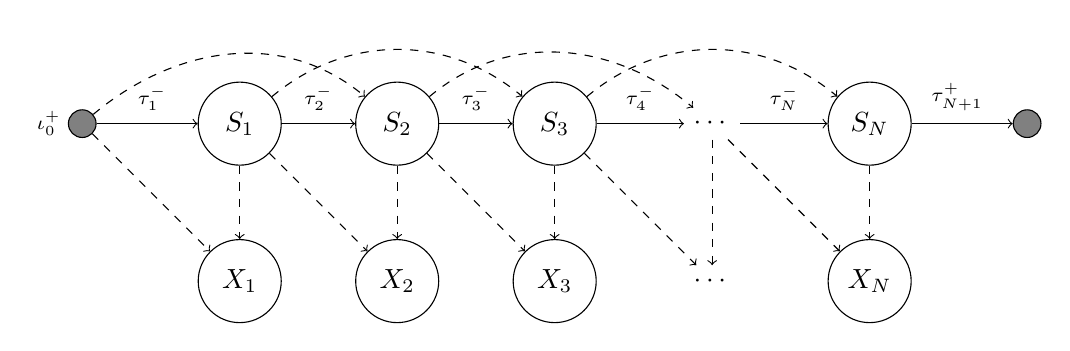
\begin{tikzpicture}[cnode/.style={draw,circle,minimum size=3em,inner sep=3pt}, onode/.style={fill=black!50, draw,circle,minimum size=1em}]
    \node (0i) at (-0.7,0) [right] {$\stackrel{\iota_0^+}{}$};
    \node[onode] (0) at (0,0) {};
    \node[cnode] (1) at (2,0) {$S_1$};
    \node[cnode] (1x) at (2,-2) {$X_1$};
    \node[cnode] (2) at (4, 0)  {$S_2$};
    \node[cnode] (2x) at (4, -2)  {$X_2$};
    \node[cnode] (3) at (6, 0)  {$S_3$};
    \node[cnode] (3x) at (6, -2)  {$X_3$};
    \node (t) at (8, 0) {$\cdots$};
    \node (tx) at (8, -2) {$\cdots$};
    \node[cnode] (N) at (10, 0)  {$S_N$};
    \node[cnode] (Nx) at (10, -2)  {$X_N$};
    \node[onode] (tt) at (12, 0) {};

    \draw[->] (0) edge node [pos=0.55, above] {$\stackrel{\tm_1}{}$}  (1) ;
    \draw[->] (1) edge node [pos=0.5, above] {$\stackrel{\tm_2}{}$}  (2) ;
    \draw[->] (2) edge node [pos=0.5, above] {$\stackrel{\tm_3}{}$}  (3) ;
    \draw[->] (3) edge node [pos=0.5, above] {$\stackrel{\tm_4}{}$}  (t) ;
    \draw[->] (t) edge node [pos=0.5, above] {$\stackrel{\tm_N}{}$}  (N) ;
    \draw[->] (N) edge node [pos=0.45, above] {$\stackrel{\tau^+_{N+1}}{}$} (tt) ;

   \begin{scope}[dashed]
    \draw[->] (0) to[out=40,in=140] (2) ;
    \draw[->] (1) to[out=40,in=140] (3) ;
    \draw[->] (2) to[out=40,in=140] (t) ;
    \draw[->] (3) to[out=40,in=140] (N) ;
   \end{scope}

   \begin{scope}[dashed]
    \draw[->] (0) to (1x) ;
    \draw[->] (1) to (1x) ;
    \draw[->] (1) to (2x) ;
    \draw[->] (2) to (2x) ;
    \draw[->] (2) to (3x) ;
    \draw[->] (3) to (3x) ;
    \draw[->] (3) to (tx) ;
    \draw[->] (t) to (tx) ;
    \draw[->] (t) to (Nx) ;
    \draw[->] (N) to (Nx) ;
   \end{scope}

\end{tikzpicture}
\caption{\em An example ($m=2, \ell=2$) of an order-$(m,\ell)$ stateful Markov process of random length $N$,
 where state $S_t$ depends on (at most) $m$ previous states, and value $X_t$ depends upon $S_t$ and 
(at most) $\ell-1$ previous states.}
\label{fig:stateful-m-ell}
\end{figure}
The corresponding likelohood model of this order-$(m,\ell)$ state--value sequence process is ?????????????????????????????.


**********************************************
Consider the first-order Markov process $R$ depicted in Figure~\ref{fig:simple-random-process}.
Suppose now that the random variable $R_t$ at stage $t$ can be decomposed into the tuple
$R_t=(S_t,X_t)$, where $S_t$ is a random {\em state} variable taking values $s_t\in{\cal S}$, and $X_t$
is a random {\em value} variable taking values $x_t\in{\cal X}$.
We make the common presumption that the stage transitions in the sequence generating process are entirely between states, e.g.\ from $S_{t-1}$ to $S_t$.
It follows from causaion that the value is generated after the state has been determined, i.e.\ $X_t$ depends upon $S_t$.
Keeping to the first-order Markov interpretation of stage-to-stage dependencies leads to
the {\em stateful} process depicted in Figure~\ref{fig:stateful-process}, with full cross-dependencies between $(S_t,X_t)$ and
$(S_{t+1},X_{t+1})$. Note that the restriction to order $m=1$ is not really onerous --  we may at any time generalise the process by inserting additional (dashed) dependencies
(viz Figure~\ref{fig:causal-process}).
\begin{figure}[hbt]
\centering
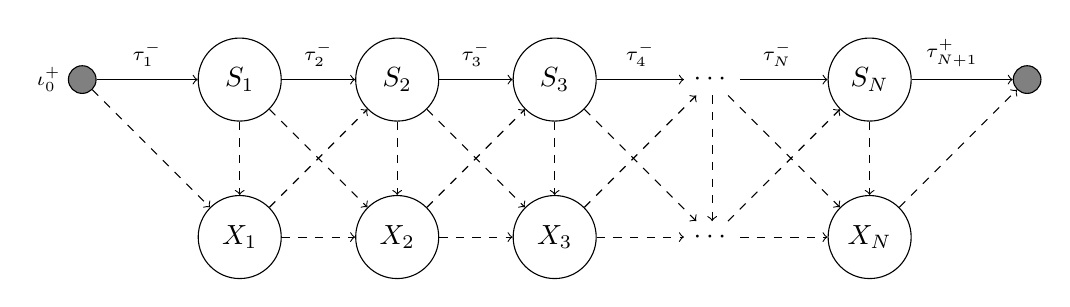
\begin{tikzpicture}[cnode/.style={draw,circle,minimum size=3em,inner sep=3pt}, onode/.style={fill=black!50, draw,circle,minimum size=1em}]
    \node (0i) at (-0.7,0) [right] {$\stackrel{\iota_0^+}{}$};
    \node[onode] (0) at (0,0) {};
    \node[cnode] (1) at (2,0) {$S_1$};
    \node[cnode] (1x) at (2,-2) {$X_1$};
    \node[cnode] (2) at (4, 0)  {$S_2$};
    \node[cnode] (2x) at (4, -2)  {$X_2$};
    \node[cnode] (3) at (6, 0)  {$S_3$};
    \node[cnode] (3x) at (6, -2)  {$X_3$};
    \node (t) at (8, 0) {$\cdots$};
    \node (tx) at (8, -2)  {$\cdots$};
    \node[cnode] (N) at (10, 0)  {$S_N$};
    \node[cnode] (Nx) at (10, -2)  {$X_N$};
    \node[onode] (tt) at (12,0) {};

    \draw[->] (0) edge node [pos=0.5, above] {$\stackrel{\tm_1}{}$}  (1) ;
    \draw[->] (1) edge node [pos=0.5, above] {$\stackrel{\tm_2}{}$}  (2) ;
    \draw[->] (2) edge node [pos=0.5, above] {$\stackrel{\tm_3}{}$}  (3) ;
    \draw[->] (3) edge node [pos=0.5, above] {$\stackrel{\tm_4}{}$}  (t) ;
    \draw[->] (t) edge node [pos=0.7, above left] {$\stackrel{\tm_N}{}$} (N) ;
    \draw[->] (N) edge node [pos=0.75, above left] {$\stackrel{\tau^+_{N+1}}{}$} (tt) ;

   \begin{scope}[dashed]
    \draw[->] (0) to (1x) ;
    \draw[->] (1) to (1x) ;
    \draw[->] (1) to (2x) ;
    \draw[->] (1x) to (2) ;
    \draw[->] (1x) to (2x) ;
    \draw[->] (2) to (2x) ;
    \draw[->] (2) to (3x) ;
    \draw[->] (2x) to (3) ;
    \draw[->] (2x) to (3x) ;
    \draw[->] (3) to (3x) ;
    \draw[->] (3) to (tx) ;
    \draw[->] (3x) to (tx) ;
    \draw[->] (3x) to (t) ;
    \draw[->] (t) to (Nx) ;
    \draw[->] (t) to (tx) ;
    \draw[->] (N) to (Nx) ;
    \draw[->] (tx) to (N) ;
    \draw[->] (tx) to (Nx) ;
    \draw[->] (Nx) to (tt) ;
   \end{scope}
\end{tikzpicture}
\caption{\em A first-order Markov process for generating complete state--value sequences of random length $N$,
with explicit cross-dependencies between adjacent stages.}
\label{fig:stateful-process}
\end{figure}

For convenience, we may notionally separate the observed states at each stage from the observed values at the corresponding stages, by loosely defining
\begin{eqnarray}
\vr & = & (r_1,r_2,\ldots,r_n)
\nonumber\\& = & 
((s_1,x_1),(s_2,x_2),\ldots,(s_n,x_n))
\nonumber\\& \equiv & 
(s_1,\ldots,s_n)\odot (x_1,\ldots,x_n)~=~(\vs,\vx)\,.
\end{eqnarray}
Consequently, the likelihood of a stateful sequence is now given by
\begin{eqnarray}
p(\iota_0,\vs,\vx,\tau_{n+1}) & = &
p(\iota_0,\tm_1,s_1,x_1,\ldots,\tm_n,s_n,x_n,\tau_{n+1})
\nonumber\\& = &
p(\iota_0)\,p(\tm_1,s_1\,|\,\iota_0)\,p(x_1\,|\,\iota_0,\tm_1,s_1)
\nonumber\\{}&&\times
\left\{\prod_{t=2}^{n}p(\tm_t,s_t\,|\,\tm_{t-1},s_{t-1},x_{t-1})\,p(x_t\,|\,\tm_t,s_t,\tm_{t-1},s_{t-1},x_{t-1})\right\}
\nonumber\\&&{}\times
p(\tau_{n+1}\,|\,\tm_n,s_n,x_n)
%
%p({\iota},\vec{s},\vec{x},{\tau}) & = & 
%p(\iota_0\!=\!{\iota})\,p(\tau_1\!=\!0\,|\,\iota_0\!=\!{\iota})
%\,p(S_1\!=\!s_1\,|\,\iota_0\!=\!{\iota},\tau_1\!=\!0)
%\nonumber\\&&{}\times
%\,p(X_1\!=\!x_1\,|\,S_1\!=\!s_1,\iota_0\!=\!{\iota},\tau_1\!=\!0)
%\nonumber\\&&
%{}\times\left\{\prod_{t=2}^{n}p(\tau_t\!=\!0\,|\,S_{t-1}\!=\!s_{t-1},X_{t-1}\!=\!x_{t-1})\right.
%\nonumber\\&&\hspace*{10mm}{}\times\left.
%\,p(S_t\!=\!s_t\,|\,\tau_t\!=\!0,S_{t-1}\!=\!s_{t-1},X_{t-1}\!=\!x_{t-1})\right.
%\nonumber\\&&\hspace*{10mm}{}\times\left.\rule{0pt}{6mm}
%\,p(X_t\!=\!x_t\,|\,S_t\!=\!s_t,S_{t-1}\!=\!s_{t-1},X_{t-1}\!=\!x_{t-1})\right\}
%\nonumber\\&&
%{}\times p(\tau_{n+1}\!=\!{\tau}\,|\,S_n\!=\!s_n,X_n\!=\!x_n)
%\nonumber\\
%&=&
%p({\iota})\,p(\tm_1\,|\,{\iota})
%\,p(s_1\,|\,{\iota},\tm_1)
%\,p(x_1\,|\,s_1,{\iota},\tm_1)
%\nonumber\\&&
%{}\times\left\{\prod_{t=2}^{n}p(\tm_t\,|\,s_{t-1},x_{t-1})
%\,p(s_t\,|\,\tm_t,s_{t-1},x_{t-1})
%\,p(x_t\,|\,s_t,s_{t-1},x_{t-1})\right\}
%\nonumber\\&&
%{}\times p({\tau}\,|\,s_n,x_n)
\,.
\end{eqnarray}
Conditioning the state $S_t$ on both the previous state $S_{t-1}$ and its value $X_{t-1}$
can be useful in some circumstances, e.g.\ in sequence classification problems.
However, due to the increased complexity of such models, it is more usual to further restrict the stateful process
by also imposing the first-order Markov assumption at the level
of the state--value dependencies themselves. In terms of the process depicted in Figure~\ref{fig:stateful-process},
this means retaining only direct node-to-node dependencies, rather than stage-to-stage dependencies.
This restricted process is depicted in Figure~\ref{fig:stateful-1-process}.
\begin{figure}[hbt]
\centering
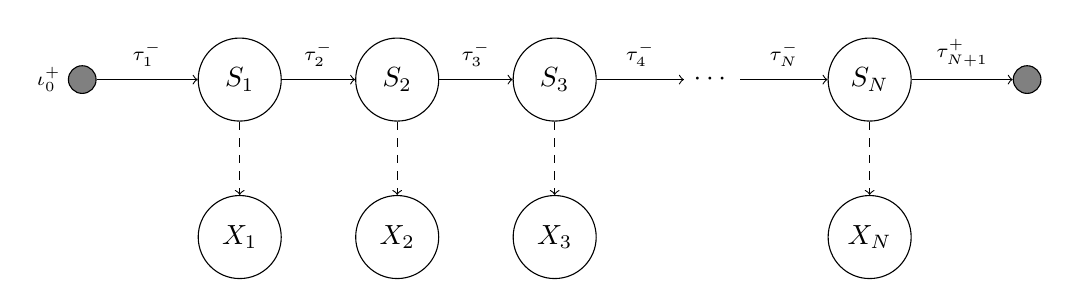
\begin{tikzpicture}[cnode/.style={draw,circle,minimum size=3em,inner sep=3pt}, onode/.style={fill=black!50, draw,circle,minimum size=1em}]
    \node (0i) at (-0.7,0) [right] {$\stackrel{\iota_0^+}{}$};
    \node[onode] (0) at (0,0) {};
    \node[cnode] (1) at (2,0) {$S_1$};
    \node[cnode] (1x) at (2,-2) {$X_1$};
    \node[cnode] (2) at (4, 0)  {$S_2$};
    \node[cnode] (2x) at (4, -2)  {$X_2$};
    \node[cnode] (3) at (6, 0)  {$S_3$};
    \node[cnode] (3x) at (6, -2)  {$X_3$};
    \node (t) at (8, 0) {$\cdots$};
    \node[cnode] (N) at (10, 0)  {$S_N$};
    \node[cnode] (Nx) at (10, -2)  {$X_N$};
    \node[onode] (tt) at (12,0) {};

    \draw[->] (0) edge node [pos=0.5, above] {$\stackrel{\tm_1}{}$}  (1) ;
    \draw[->] (1) edge node [pos=0.5, above] {$\stackrel{\tm_2}{}$}  (2) ;
    \draw[->] (2) edge node [pos=0.5, above] {$\stackrel{\tm_3}{}$}  (3) ;
    \draw[->] (3) edge node [pos=0.5, above] {$\stackrel{\tm_4}{}$}  (t) ;
    \draw[->] (t) edge node [pos=0.5, above] {$\stackrel{\tm_N}{}$}  (N) ;
    \draw[->] (N) edge node [pos=0.5, above] {$\stackrel{\tau^+_{N+1}}{}$}  (tt) ;

   \begin{scope}[dashed]
    \draw[->] (1) to (1x) ;
    \draw[->] (2) to (2x) ;
    \draw[->] (3) to (3x) ;
    \draw[->] (N) to (Nx) ;
   \end{scope}
\end{tikzpicture}
\caption{\em A first-order Markov process for generating complete state--value  sequences of random length $N$.}
\label{fig:stateful-1-process}
\end{figure}
The corresponding sequence model is now given by
\begin{eqnarray}
p(\iota_0,\vs,\vx,\tau_{n+1}) & = &
%p(\iota_0,\tm_1,s_1,x_1,\ldots,\tm_n,s_n,x_n,\tau_{n+1})
%\nonumber\\& = &
p(\iota_0)\,p(\tm_1,s_1\,|\,\iota_0)\,p(x_1\,|\,\tm_1,s_1)
\nonumber\\{}&&\times
\left\{\prod_{t=2}^{n}p(\tm_t,s_t\,|\,\tm_{t-1},s_{t-1})\,p(x_t\,|\,\tm_t,s_t)\right\}
%\nonumber\\&&{}\times
\,p(\tau_{n+1}\,|\,\tm_n,s_n)\,.
\label{eq:stateful-1-model}
\end{eqnarray}


\subsection{Hidden State Sequences}\label{sec:hidden-state}

A special case of the stateful Markov sequence process is the so-called {\em hidden Markov model} (HMM), where the values of the state sequence $\vs$ are
entirely unobserved (and perhaps unobservable). However, more generally we have to consider the possibility that the values of any of the random variables 
$\iota_0$, $S_t$, $X_t$ and $\tau_{n+1}$ might or might not have been observed in practice. The extension of equation~\eqref{eq:pr:discrete} is straightforward
for discrete\footnote{Recall from Section~\ref{sec:missing-values} that the continuous analogue is readily derivable from the discrete model.} states and values, namely
\begin{eqnarray}
p(\ui,\uvs,\uvx,\ut) 
& = & 
\sum_{\iota_0=0}^{1}\delta(\iota_0\!=\!\ui)
\sum_{s_1\in{\cal S}} \delta(s_1\!=\!\us_1)
\sum_{x_1\in{\cal X}} \delta(x_1\!=\!\ux_1)
\cdots\sum_{s_n\in{\cal S}} \delta(s_n\!=\!\us_n)
\sum_{x_n\in{\cal X}} \delta(x_n\!=\!\ux_n)
\nonumber\\&&
\,\sum_{\tau_{n+1}=0}^{1}\delta(\tau_{n+1}\!=\!\ut)
\,p(\iota_0,\tm_1,s_1,x_1,\ldots,\tm_n,s_n,x_n,\tau_{n+1})\,.
\label{eq:pr:discrete:state-value}
\end{eqnarray}
This calculation can be simplified further under the first-order state--value model~\eqref{eq:stateful-1-model}.
For example, the fact that an $x_t$ is unobserved, i.e.\ $\ux_t=*$, is easily handled, since $X_t$ depends only on $S_t$ in stage $t$. Specifically, the marginalisation over $x_t\in{\cal X}$ affects exactly one term in the model, and consequently we may
define $p(*\,|\,\tm_t,s_t)=p(X_t\!=\!*\,|\,\tau_t\!=\!0,S_t\!=\!s_t)=1$; hence $p(\underline{x}_t\,|\,\tm_t,s_t)$ is well defined. Note that this simplification is only applicable when
$X_t$ does not depend upon any earlier $X_{t-k}$; such higher-order dependencies will require the more general handling of marginalisation above.

Similarly, if the termination marker $\tau_{n+1}$ is unobserved, i.e.\ $\ut=*$, then 
 $p(\ut\,|\,\tm_n,s_n)$ is still well defined if we let
$p(\tau_{n+1}=*\,|\,\tau_n\!=\!0,S_n\!=\!s_n)=1$.
However, if the initiation marker $\iota_0$ is unobserved, i.e.\ $\ui=*$, then the marginalisation is more difficult
because $\iota_0$ also conditions $S_1$ via $p(S_1\,|\,\iota_0,\tau_1)$. To allow for this, we define (for order $m=1$) that
\begin{eqnarray}
 p(\ui,\tm_1,s_1) & = & \sum_{\iota=0}^{1}\delta(\iota\!=\!\ui) \,p(\iota_0)\,p(\tm_1,s_1\,|\,\iota_0)\,,
\end{eqnarray}
such that
\begin{eqnarray}
p(\ui,\vs,\uvx,\ut) & = & 
p(\ui,\tm_1,s_1)
\,p(\ux_1\,|\,\tm_1,s_1)
\left\{\prod_{t=2}^{n}p(\tm_t,s_t\,|\,\tm_{t-1},s_{t-1})
\,p(\ux_t\,|\,s_t)\right\}
\,p(\ut\,|\,s_n)
\,.
\label{eq:stateful-1-model:hidden-markers}
\end{eqnarray}
Hence, we obtain
\begin{eqnarray}
p(\ui,\uvs,\uvx,\ut) & = & 
\sum_{s_1\in{\cal S}} \delta(s_1\!=\!\us_1)
\cdots\sum_{s_n\in{\cal S}} \delta(s_n\!=\!\us_n)
\,p(\ui,\vs,\uvx,\ut)\,.
\end{eqnarray}
Note that the conventional HMM formulation is obtained by dropping the $\ui$, $\uvs$ and $\ut$ terms and the $\delta(\cdot)$ indicators.

\subsection{Stateful Forward--Backward Algorithm}\label{sec:forward-backward:stateful}

Under the conventions discussed in the previous section, the forward--backward algorithm for order $m$ stateful Markov sequences takes the form

The observed sequence model~\eqref{eq:state-marg} can be efficiently evaluated by marginalising over the state of each stage
in turn, using a modification of the {\em forward--backward algorithm} to include knowledge of
sequence initiation and termination.
 The forward pass involves first summing over all terms containing $s_1$, then over all remaining terms containing $s_2$,
and so on up to $s_n$. This is equivalent to evaluating the reordered model
\begin{eqnarray}
   p(\ui,\underline{\vec{s}},\underline{\vec{x}},\ut) 
& = & 
   \left\{\sum_{s_n\in{\cal S}}\delta(s_n\!=\!\underline{s}_n)
\cdots
\right\{\sum_{s_2\in{\cal S}}\delta(s_2\!=\!\underline{s}_2)
\nonumber\\&&
\hspace*{10mm}{}
\left\{\sum_{s_1\in{\cal S}}\delta(s_1\!=\!\underline{s}_1)\,
p(\ui,\tm_1,s_1)\,p(\underline{x}_1\,|\,s_1)\,p(\tm_2\,|\,s_1)\,p(s_2\,|\,\tm_2,s_1)\right\}
\nonumber\\&&
\left.\rule{0pt}{6mm}
p(\underline{x}_{2}\,|\,s_2)\,p(\tm_3\,|\,s_2)\,p(s_3\,|\,\tm_3,s_2)\right\}
\cdots
\left.\rule{0pt}{6mm}\,p(\underline{x}_{n}\,|\,s_n)
\,p(\ut\,|\,s_n)\right\}
\,.
\label{eq:forward}
\end{eqnarray}
 The forward pass commences with the first stage of the sequence, and includes the inner terms that are dependent on state $s_1$, namely
\begin{eqnarray}
  \alpha_1(s_1) & = & p(\ui,\tm_1,s_1)\,p(\underline{x}_1\,|\,s_1)
\nonumber\\&=&
p(\ui,\tm_1,s_1,\underline{x}_1)~\equiv~p(\ui,\underline{\vec{s}}_0\circ s_1,\underline{\vec{x}}_1)\,,
\label{eq:alpha_1}
\end{eqnarray}
where the operator `$\circ$' indicates the concatenation of either two elements, two sequences or an element and a sequence, to form a longer sequence.
Recall that $\underline{\vec{s}}_0$ is an empty sequence.

The next step of the forward pass now moves on to the second stage and includes terms dependent on state $s_2$ at that stage:
\begin{eqnarray}
  \alpha_2(s_2) & = & 
\left\{\sum_{s_1\in{\cal S}}\delta(s_1\!=\!\underline{s}_1)\,
\alpha_1(s_1)\,p(\tm_2\,|\,s_1)\,p(s_2\,|\,\tm_2,s_1)\right\}
\,p(\underline{x}_2\,|\,s_2)
\nonumber\\&=&
\left\{\sum_{s_1\in{\cal S}}\delta(s_1\!=\!\underline{s}_1)\,
p(\ui,\tm_1,s_1,\underline{x}_1)\,p(\tm_2\,|\,s_1)\,p(s_2\,|\,\tm_2,s_1)\right\}
\,p(\underline{x}_2\,|\,s_2)
\nonumber\\&=&
\left\{\sum_{s_1\in{\cal S}}\delta(s_1\!=\!\underline{s}_1)\,
p(\ui,\tm_1,s_1,\underline{x}_1,\tm_2,s_2)\right\}
\,p(\underline{x}_2\,|\,s_2)
\nonumber\\&=&
p(\ui,\tm_1,\underline{s}_1,\underline{x}_1,\tm_2,s_2)\,p(\underline{x}_2\,|\,s_2)
\nonumber\\&=&
p(\ui,\tm_1,\underline{s}_1,\underline{x}_1,\tm_2,s_2,\underline{x}_2)
~\equiv~p(\ui,\underline{\vec{s}}_1\circ s_2,\underline{\vec{x}}_2)
\,.
\label{eq:alpha_2}
\end{eqnarray}
Recursively, the last step of the forward pass stops at the $n$-th stage, giving
\begin{eqnarray}
  \alpha_n(s_n) & = & 
\left\{\sum_{s_{n-1}\in{\cal S}}\delta(s_{n-1}\!=\!\underline{s}_{n-1})\,
\alpha_{n-1}(s_{n-1})\,p(\tm_n\,|\,s_{n-1})\,p(s_n\,|\,\tm_n,s_{n-1})\right\}
\,p(\underline{x}_n\,|\,s_n)
\nonumber\\&\equiv&
p(\ui,\underline{\vec{s}}_{n-1}\circ s_n,\underline{\vec{x}}_{n-1})\,p(\underline{x}_n\,|\,s_n)
~=~p(\ui,\underline{\vec{s}}_{n-1}\circ s_n,\underline{\vec{x}}_n)
\,.
\label{eq:alpha_n}
\end{eqnarray}
The remaining terms then give the observed joint likelihood
\begin{eqnarray}
   p(\ui,\underline{\vec{s}},\underline{\vec{x}},\ut) 
& = & 
   \sum_{s_n\in{\cal S}}\delta(s_n\!=\!\underline{s}_n)\,\alpha_n(s_n)\,p(\ut\,|\,s_n)\,.
\label{eq:alpha_n_beta_n}
\end{eqnarray}

Conversely, the backaward pass involves first summing over all terms containing $s_n$,
then over all remaining terms containing $s_{n-1}$, and so on down $s_1$.
This is equivalent to evaluating the reordered model
\begin{eqnarray}
   p(\ui,\underline{\vec{s}},\underline{\vec{x}},\ut) 
& = & 
   \left\{\sum_{s_1\in{\cal S}}\delta(s_1\!=\!\underline{s}_1)\,
p(\ui,\tm_1,s_1)\,p(\underline{x}_1\,|\,s_1)\,p(\tm_2\,|\,s_1)\,
\cdots\right.
\nonumber\\&&
\;\;\;\left\{\sum_{s_{n-1}\in{\cal S}}\delta(s_{n-1}\!=\!\underline{s}_{n-1})\,
p(s_{n-1}\,|\,\tm_{n-1},s_{n-2})\,p(\underline{x}_{n-1}\,|\,s_{n-1})\,p(\tm_n\,|\,s_{n-1})\right.
\nonumber\\&&
\hspace*{4mm}
\left.\rule{0pt}{7mm}\left\{\sum_{s_n\in{\cal S}}\delta(s_n\!=\!\underline{s}_n)\,
p(s_n\,|\,\tm_n,s_{n-1})\,p(\underline{x}_{n}\,|\,s_n)
\,p(\ut\,|\,s_n)\right\}\right\}
\cdots\left.\rule{0pt}{7mm}\right\}
\,.
\label{eq:backward}
\end{eqnarray}
The backward pass commences at the end of the sequence with the termination term that depends on state $s_n$, namely 
\begin{eqnarray}
  \beta_n(s_n) & = & p(\ut\,|\,s_n)\,.
\label{eq:_beta_n}
\end{eqnarray}
The next step in the backward pass then moves backward to the $n$-th stage and incorporates the terms that depend on state $s_{n-1}$, including the
non-terminating transition from $s_{n-1}$ to $s_n$
\begin{eqnarray}
  \beta_{n-1}(s_{n-1}) & = &
p(\tm_n\,|\,s_{n-1})\,\left\{\sum_{s_n\in{\cal S}}\delta(s_n\!=\!\underline{s}_n)\,
p(s_n\,|\,\tm_n,s_{n-1})\,p(\underline{x}_{n}\,|\,s_n)
\,\beta_n(s_n)\right\}
\nonumber\\&=&
p(\tm_n\,|\,s_{n-1})\,\left\{\sum_{s_n\in{\cal S}}\delta(s_n\!=\!\underline{s}_n)\,
p(s_n\,|\,\tm_n,s_{n-1})\,p(\underline{x}_{n}\,|\,s_n)
\,p(\ut\,|\,s_n)\right\}
\nonumber\\&=&
p(\tm_n\,|\,s_{n-1})\,\left\{\sum_{s_n\in{\cal S}}\delta(s_n\!=\!\underline{s}_n)\,
p(s_n,\underline{x}_{n},\ut\,|\,\tm_n,s_{n-1})\right\}
\nonumber\\&=&
p(\tm_n\,|\,s_{n-1})\,p(\underline{s}_n,\underline{x}_n,\ut\,|\,\tm_n,s_{n-1})
\nonumber\\&=&
p(\tm_n,\underline{s}_n,\underline{x}_n,\ut\,|\,s_{n-1})
~\equiv~p(\circ\underline{\rvec{s}}_n,\underline{\rvec{x}}_n,\ut\,|\,s_{n-1})\,.
\end{eqnarray}
Observe that we have explicitly included the concatenation operator to indicate the presence of $\tm_{n}$. 
Symbolically, we may write $p(\vr)=p(\vr_t\circ\rvec{r}_{t+1})=p(\vr_t\circ)p(\rvec{r}_{t+1})=p(\vr_t)p(\circ\rvec{r}_{t+1})$.

Recursively, the last step of the backward pass reaches the first stage, giving
\begin{eqnarray}
  \beta_{1}(s_{1}) & = &
p(\tm_2\,|\,s_{1})\,\sum_{s_2\in{\cal S}}\delta(s_2\!=\!\underline{s}_2)\,
p(s_2\,|\,\tm_2,s_{1})\,p(\underline{x}_{2}\,|\,s_2)
\,\beta_2(s_2)
\nonumber\\&=&
p(\tm_2\,|\,s_{1})\,
p(\underline{s}_2,\underline{x}_2,\tm_3,\ldots,\underline{s}_n,\underline{x}_n,\ut\,|\,\tm_2,s_{1})
\nonumber\\&\equiv&
p(\circ\underline{\rvec{s}}_2,\underline{\rvec{x}}_2,\ut\,|\,s_{1})\,.
\end{eqnarray}
The remaining terms then give the observed likelihood
\begin{eqnarray}
   p(\ui,\underline{\vec{s}},\underline{\vec{x}},\ut) 
& = & 
   \sum_{s_1\in{\cal S}}\delta(s_1\!=\!\underline{s}_1)\,p(\ui,\tm_1,s_1)\,\beta_1(s_1)\,.
\end{eqnarray}
In general, we obtain
\begin{eqnarray}
   p(\ui,\underline{\vec{s}},\underline{\vec{x}},\ut) 
& = & 
   \sum_{s_t\in{\cal S}}\delta(s_t\!=\!\underline{s}_t)\,
   p(\ui,\underline{\vec{s}}_{t-1}\circ s_t\circ\underline{\rvec{s}}_{t+1},
\underline{\vec{x}}_t\circ\underline{\rvec{x}}_{t+1},\ut) 
\nonumber\\&=&
   \sum_{s_t\in{\cal S}}\delta(s_t\!=\!\underline{s}_t)\,
p(\ui,\underline{\vec{s}}_{t-1}\circ s_t,\underline{\vec{x}}_t)
\,p(\circ\underline{\rvec{s}}_{t+1},\underline{\rvec{x}}_{t+1},\ut\,|\,s_{t})
\nonumber\\&=&
   \sum_{s_t\in{\cal S}}\delta(s_t\!=\!\underline{s}_t)\,\alpha_t(s_t)\,\beta_t(s_t)\,,
\end{eqnarray}
for all $t=1,2,\ldots,n$. The case for $t=n$ comes from equations~\eqref{eq:alpha_n_beta_n} and \eqref{eq:_beta_n}; alternatively, recall that $\rvec{r}_{n+1}$ is an empty sequence.

%%%%%%%%%%%%%%%%%%%%%%%%%%%%%%%%%%%%%%%%%%%%%%%%%%%%%%%%%%%%%%%%%%%%
\section{Discrete-state Sequence Models}\label{sec:discrete-state}

Consider the stateful, first-order Markov process depicted by Figure~\ref{fig:stateful-1-process}.
Let us now restrict our attention to the class of corresponding sequence models where
the state $S_t$ at any stage $t$ may now only take {\em discrete} values in the set 
${\cal S}=\{\sigma_1,\sigma_2,\ldots,\sigma_S\}$.
Hence, the sequence of states may arbitrarily be specified as $\vec{s}=(\sigma_{i_1},\sigma_{i_2},\ldots,\sigma_{i_n})$,
where each $i_t\in\{1,2,\ldots,S\}$.
In the event that a particular state $S_t$ is unobserved, we say that the state is {\em missing} or {\em hidden},
and denote $i_t=*$ and $s_t=*$. In the situation where all values of $\vec{s}$ are unobserved,
the sequence model~\eqref{eq:stateful-1-model} is known as a {\em hidden-state Markov model} (HMM).

The sequence model~\eqref{eq:stateful-1-model}
may now be explicitly conditioned on a general parameter $\theta$
that governs the various discrete state distributions. Each term in the model depends directly on the stage index $t$ and 
indirectly on the state index $i_t$. 
Furthermore, each term represents either the initial state, the terminal state, or the non-terminal transitions
between states at adjacent stages. Hence, let $\theta=(\Pi,\Gamma,\Omega)$, 
such that the probability of an arbitrary, observed\footnote{We assume that all observed sequences are non-zero in length,
since zero-length sequences are typically unobservable unless the generating process explicitly signals the start
and end of each sequence. The modelling of zero-length sequences will require an extra parameter.} sequence (with no hidden states) is given by
\begin{eqnarray}
p(\ui,\vec{s},\vec{x},\ut\,|\,\theta) & = & \pi_{\ui,1,i_1}\,o_{1,i_1}(x_1)\left\{\prod_{t=1}^{n-1}\omega_{0,t,i_t}\,\Gamma_{t,i_t,i_{t+1}}\,o_{t+1,i_{t+1}}(x_{t+1})
\right\}\,\omega_{\ut,n,i_n}
\,.
\label{eq:p_s_x_g_theta}
\end{eqnarray}
The initial state $S_1$ of the sequence at stage $t=1$ is governed by the parameter $\vec{\pi}$, where
\begin{eqnarray}
  \pi_{0,t,i} & = & p(\iota_{t-1}\!=\!0\,|\,\theta)\,p(\tau_t\!=\!0\,|\,\iota_{t-1}\!=\!0,\theta)
      \,p(S_t\!=\!\sigma_{i}\,|\,\iota_{t-1}\!=\!0,\tau_t\!=\!0,\theta)\,,
\\
  \pi_{1,t,i} & = & p(\iota_{t-1}\!=\!1\,|\,\theta)\,p(\tau_t\!=\!0\,|\,\iota_{t-1}\!=\!1,\theta)
      \,p(S_t\!=\!\sigma_{i}\,|\,\iota_{t-1}\!=\!1,\tau_t\!=\!0,\theta)\,,
\end{eqnarray}
and
\begin{eqnarray}
  \pi_{*,t,i} & = & p(\iota_{t-1}\!=\!*\,|\,\theta)\,p(\tau_t\!=\!0\,|\,\iota_{t-1}\!=\!*,\theta)
      \,p(S_t\!=\!\sigma_{i}\,|\,\iota_{t-1}\!=\!*,\tau_t\!=\!0,\theta)
\nonumber\\& = &
  p(\tau_t\!=\!0,S_t\!=\!\sigma_i\,|\,\theta)~=~\pi_{0,t,i}+\pi_{1,t,i}\,.
\label{eq:pi:*}
\end{eqnarray}
Observe that each state $S_t$ for $t>1$ is a non-initial state, governed by $\pi_{0,t,i_t}$. However, such terms do
not explicitly appear in model~\eqref{eq:p_s_x_g_theta}, except if $\ui\ne 1$, 
since they are already accounted for by the state transitions.
These implicit terms become important when it comes to parameter estimation (see Section~\ref{sec:estimate-known}).

The terminal state $S_n$ at stage $t=n$ is likewise governed by the parameter $\vec{\omega}$, where
\begin{eqnarray}
  \omega_{0,t,i} & = & p(\tau_{t+1}\!=\!0\,|\,S_t\!=\!\sigma_{i},\theta)\,,
\\
  \omega_{1,t,i} & = & p(\tau_{t+1}\!=\!1\,|\,S_t\!=\!\sigma_{i},\theta)\,,
\end{eqnarray}
and
\begin{eqnarray}
  \omega_{*,t,i} & = & p(\tau_{t+1}\!=\!*\,|\,S_t\!=\!\sigma_{i},\theta)
~=~\omega_{0,t,i}+\omega_{1,t,i}~=~1\,.
\end{eqnarray}
Observe that each state $S_t$ for $t<n$ is a non-terminal state, and is explicitly modelled by the term
$\omega_{0,t,i_t}$.

Lastly, the permissible transitions between the states $S_t$ and $S_{t+1}$ of consecutive stages $t$ and $t+1$ are governed by
the parameter $\Gamma$, where
\begin{eqnarray}
  \Gamma_{t,i,j} & = & p(S_{t+1}\!=\!\sigma_{j}\,|\,S_t\!=\!\sigma_{i},\tau_{t+1}\!=\!0,\theta)\,.
\end{eqnarray}
Note that the model also includes the likelihood of each observed value $x_t$ at stage $t$, for $t=1,2,\ldots,n$.
This so-called {\em data likelihood} is governed by the separate model
\begin{eqnarray}
  o_{t,i}(x) & = & p(X_t\!=\!x\,|\,S_t\!=\!\sigma_{i},\theta) \hspace*{5mm}\forall x\in{\cal X}\,.
\end{eqnarray}
We do not, however, explicitly declare the parameterisation structure of this likelihood model (see Section~\ref{sec:discrete-x} for a plausible model if $X_t$ takes discrete values). 
It suffices for our calculations that each $o_{t,i_t}(x_t)$ is available when required.

Finally, note that in the situtation where any state in the observed state sequence $\vec{s}$ is hidden, we have to marginalise model~\eqref{eq:p_s_x_g_theta} over each such missing state. Hence, in general, we may define
\begin{eqnarray}
   p(\ui,\vec{s},\vec{x},\ut\,|\,\theta) 
& = & 
   \sum_{i_1'=1}^{S}\delta(i_1'\!=\!i_1)\sum_{i_2'=1}^{S}\delta(i_2'\!=\!i_2)\cdots\sum_{i_n'=1}^{S}\delta(i_n'\!=\!i_n)\,
\nonumber\\&&\hspace*{10mm}\pi_{\ui,1,i_1'}\,o_{1,i_1'}(x_1)\,
\left\{\prod_{t=1}^{n-1}\omega_{0,t,i_t'}\,\Gamma_{t,i_t',i_{t+1}'}\,o_{t+1,i_{t+1}'}(x_{t+1})
\right\}\,\omega_{\ut,n,i_n'}
\,,
\label{eq:p_s_x_g_theta:gen}
\end{eqnarray}
where $\delta(\cdot)$ is an indicator function taking the value $1$ (or $0$) if its argument is true (or false).
Note that if $S_t$ is a hidden state, then $i_t=*$ and $\delta(i_t'\!=\!*)=1$ for all $i_t'\in\{1,2,\ldots,S\}$; otherwise, the summation over $i_t'$ collapses to the observed value $i_t$.
The observation likelihood given by model~\eqref{eq:p_s_x_g_theta:gen} can be efficiently computed by an
extension of the forward--backward algorithm, described in the next section.

\subsection{Modified Forward--Backward Algorithm}\label{sec:forward-backward}

The sequence model~\eqref{eq:p_s_x_g_theta:gen} can be efficiently evaluated by marginalising over the state of each stage
in turn, using a modification of the {\em forward--backward algorithm} to include knowledge of
sequence initiation and termination.
 The forward pass involves first summing over all terms containing $i_1'$, then over all remaining terms containing $i_2'$,
and so on up to summing over $i_n'$. This is equivalent to evaluating the reordered model
\begin{eqnarray}
   p(\ui,\vec{s},\vec{x},\ut\,|\,\theta) 
& = & 
   \left\{\sum_{i_n'=1}^{S}\delta(i_n'\!=\!i_n)
%\left\{\sum_{i_{n-1}'=1}^{S}\delta(i_{n-1}'\!=\!i_{n-1})\right.
\cdots
\right\{\sum_{i_2'=1}^{S}\delta(i_2'\!=\!i_2)
\nonumber\\&&
\hspace*{10mm}{}\times
\left\{\sum_{i_1'=1}^{S}\delta(i_1'\!=\!i_1)\,
\pi_{\ui,1,i_1'}\,o_{1,i_1'}(x_1)\,\omega_{0,1,i_1'}\,\Gamma_{1,i_1',i_{2}'}\right\}
\nonumber\\&&
\left.\rule{0pt}{7mm}
o_{2,i_{2}'}(x_{2})\omega_{0,2,i_{2}'}\,\Gamma_{2,i_{2}',i_{3}'}\right\}
\cdots
%\left.\rule{0pt}{7mm}\omega_{0,n-1,i_{n-1}'}\,\Gamma_{n-1,i_{n-1}',i_{n}'}\right\}
\left.\rule{0pt}{7mm}\,o_{n,i_{n}'}(x_{n})
\,\omega_{\ut,n,i_n'}\right\}
\,.
\label{eq:forward}
\end{eqnarray}
Conversely, the backaward pass reverses the order of evaluation, first summing over all terms containing $i_n'$,
and then over all remaining terms containing $i_{n-1}'$, and so on down to summing over $i_1'$.
This is equivalent to evaluating the reordered model
\begin{eqnarray}
   p(\ui,\vec{s},\vec{x},\ut\,|\,\theta) 
& = & 
   \left\{\sum_{i_1'=1}^{S}\delta(i_1'\!=\!i_1)\,
\pi_{\ui,1,i_1'}\,o_{1,i_1'}(x_1)\,\omega_{0,1,i'_{1}}\,
\cdots\right.
\nonumber\\&&
{}\times\left\{\sum_{i_{n-1}'=1}^{S}\delta(i_{n-1}'\!=\!i_{n-1})\,
\Gamma_{n-2,i_{n-2}',i_{n-1}'}\,o_{n-1,i_{n-1}'}(x_{n-1})\,\omega_{0,n-1,i'_{n-1}}\right.
\nonumber\\&&
\hspace*{4mm}{}\times
\left.\rule{0pt}{7mm}\left\{\sum_{i_n'=1}^{S}\delta(i_n'\!=\!i_n)\,
\Gamma_{n-1,i_{n-1}',i_{n}'}\,o_{n,i_{n}'}(x_{n})
\,\omega_{\ut,n,i_n'}\right\}\right\}
\cdots\left.\rule{0pt}{7mm}\right\}
\,.
\label{eq:backward}
\end{eqnarray}

A more efficient mechanism for evaluation comes from making use of the first-order Markov dependencies.
Notionally, from the process depicted in Figure~\ref{fig:stateful-1-process}, we may arbitrarily consider the transition from 
some stage $t$ to stage $t+1$,
and partition the sequence into: (i) past values from the initial node up to and including $S_t$ and $X_t$;
and (ii) future values from $S_{t+1}$ and $X_{t+1}$ up to and including the terminal node.
Note that the termination or non-termination of stage $t$ is governed by $\tau_{t+1}$, which is
therefore a future value.
The Markov dependency then implies that the future values are conditioned only on state $S_t$
via $\tau_{t+1}$ and $S_{t+1}$.
Hence, remembering that notionally $s_t=\sigma_{i_t}$, model~\eqref{eq:p_s_x_g_theta:gen} reduces to
\begin{eqnarray}
   p(\ui,\vec{s},\vec{x},\ut\,|\,\theta) 
& = &
   \sum_{i=1}^{S}p(S_t\!=\!\sigma_{i},\ui,\vec{s},\vec{x},\ut\,|\,\theta) 
\nonumber\\& = & 
   \sum_{i=1}^{S}\delta(i\!=\!i_t)\,p(\ui,\vec{s}_{t-1}\circ\sigma_{i}\circ\rvec{s}_{t+1},\vec{x},\ut\,|\,\theta) 
\nonumber\\& = & 
   \sum_{i=1}^{S}\delta(i\!=\!i_t)\,p(\ui,\vec{s}_{t-1}\circ\sigma_{i},\vec{x}_t\,|\,\theta) 
\,p(\dn\rvec{s}_{t+1},\rvec{x}_{t+1},\ut\,|\,S_t=\sigma_{i},\theta) 
\nonumber\\& = &
  \sum_{i=1}^{S}\delta(i\!=\!i_t)\,\alpha_{t,i}\,\beta_{t,i}\,,
\label{eq:forward-backward}
\end{eqnarray}
where $\circ$ represents sequence concatenation.
The forward step $\alpha_{t,i}$ is defined as
\begin{eqnarray}
   \alpha_{t,i} & = & p(\ui,\vec{s}_{t-1}\circ\sigma_{i},\vec{x}_t\,|\,\theta) 
\nonumber\\& = &
   p(\ui,\vec{s}_{t-1}\circ\sigma_{i},\vec{x}_{t-1}\,|\,\theta) \,p(X_t\!=\!x_t\,|\,S_t\!=\!\sigma_{i_t},\theta)
\nonumber\\& = &
   \bar{\alpha}_{t,i}\,o_{t,i}(x_t)\,,
\label{eq:alpha}
\end{eqnarray}
where $\bar{\alpha}_{t,i}$ is recursively defined as
\begin{eqnarray}
   \bar{\alpha}_{t,i} & = & p(\ui,\vec{s}_{t-1}\circ\sigma_{i},\vec{x}_{t-1}\,|\,\theta) 
\nonumber\\& = &
   \sum_{j=1}^{S}p(S_{t-1}\!=\!\sigma_j,\ui,\vec{s}_{t-1}\circ\sigma_{i},\vec{x}_{t-1}\,|\,\theta) 
\nonumber\\& = &
   \sum_{j=1}^{S}\delta(j=i_{t-1})\,p(\ui,\vec{s}_{t-2}\circ\sigma_{j}\circ\sigma_{i},\vec{x}_{t-1}\,|\,\theta) 
\nonumber\\& = &
   \sum_{j=1}^{S}\delta(j=i_{t-1})\,p(\ui,\vec{s}_{t-2}\circ\sigma_{j},\vec{x}_{t-1}\,|\,\theta) 
      \,p(\tau_t\!=\!0\,|\,S_{t-1}\!=\!\sigma_j,\theta)
\nonumber\\&&
    \hspace*{5mm}{}\times\,p(S_t\!=\!\sigma_i\,|\,\tau_{t}\!=\!0,S_{t-1}\!=\!\sigma_j,\theta)
\nonumber\\& = &
   \sum_{j=1}^{S}\delta(j=i_{t-1})\,\alpha_{t-1,j}\,\omega_{0,t-1,j}\,\Gamma_{t-1,j,i}\,,
\label{eq:alpha-bar}
\end{eqnarray}
for $t=2,3,\ldots,n$. The forward pass commences with the first step
\begin{eqnarray}
  \alpha_{1,i} & = & p(\ui,S_1=\sigma_{i},X_1\!=\!x_1\,|\,\theta) 
\nonumber\\& = & 
  p(\iota_0\!=\!\ui)\,p(\tau_1\!=\!0\,|\,\iota\!=\!\ui,\theta)
\,p(S_1\!=\!\sigma_i\,|\,\iota_0\!=\!\ui,\tau_1\!=\!0,\theta)\,p(X_1\!=\!x_1\,|\,S_1\!=\!\sigma_i,\theta)
\nonumber\\& = & 
  \pi_{\ui,1,i}\,o_{1,i}(x_1)
\,.
\label{eq:alpha_1}
\end{eqnarray}
Hence, observe that $\alpha_{2,i'_2}$, is just
the entire summation over $i'_1$ from the forward model~\eqref{eq:forward}.
Also note that the standard forward pass derivation commences with the equivalent of $\pi_{*,1,i}$ and does not include the
$\delta(\cdot)$ or $\omega$ terms.

Conversely to the forward pass, the backward step $\beta_{t,i}$ is defined as
\begin{eqnarray}
   \beta_{t,i} & = & p(\dn\rvec{s}_{t+1},\rvec{x}_{t+1},\ut\,|\,S_t\!=\!\sigma_{i},\theta) 
\nonumber\\& = &
  p(\tau_{t+1}\!=\!0\,|\,S_t\!=\!\sigma_i,\theta)\,p(\rvec{s}_{t+1},\rvec{x}_{t+1},\ut\,|\,\tau_{t+1}\!=\!0,S_t\!=\!\sigma_{i},\theta) 
\nonumber\\& = &
  \omega_{0,t,i}\,\bar{\beta}_{t,i}\,,
\label{eq:beta}
\end{eqnarray}
where
\begin{eqnarray}
   \bar{\beta}_{t,i} & = & p(\rvec{s}_{t+1},\rvec{x}_{t+1},\ut\,|\,\tau_{t+1}\!=\!0,S_t\!=\!\sigma_{i},\theta) 
\nonumber\\& = &
  \sum_{j=1}^{S} p(S_{t+1}\!=\!\sigma_j,\rvec{s}_{t+1},\rvec{x}_{t+1},\ut\,|\,\tau_{t+1}\!=\!0,S_t\!=\!\sigma_{i},\theta) 
\nonumber\\& = &
  \sum_{j=1}^{S}\delta(j\!=\!i_{t+1})\, p(\sigma_j\circ\rvec{s}_{t+2},x_{t+1}\circ\rvec{x}_{t+2},\ut\,|\,\tau_{t+1}\!=\!0,S_t\!=\!\sigma_{i},\theta) 
%\nonumber\\& = &
 % \sum_{j=1}^{S}\delta(j\!=\!i_{t+1})\, p(S_{t+1}\!=\!\sigma_j,X_{t+1}\!=\!x_{t+1}\,|\,\tau_{t+1}\!=\!0,S_t\!=\!\sigma_{i},\theta) 
%\,p(\dn\rvec{s}_{t+2},\rvec{x}_{t+2},\ut\,|\,S_{t+1}\!=\!\sigma_{j},\theta) 
\nonumber\\& = & 
   \sum_{j=1}^{S}\delta(j\!=\!i_{t+1})\, p(S_{t+1}\!=\!\sigma_j\,|\,\tau_{t+1}\!=\!0,S_t\!=\!\sigma_i,\theta)
\,p(X_{t+1}=x_{t+1}\,|\,S_{t+1}\!=\!\sigma_j,\theta)
\nonumber\\&&\hspace*{5mm}{}\times
p(\dn\rvec{s}_{t+2},\rvec{x}_{t+2},\ut\,|\,S_{t+1}\!=\!\sigma_{j},\theta) 
\nonumber\\& = & 
	\sum_{j=1}^{S}\delta(j\!=\!i_{t+1})\,\Gamma_{t,i,j}\,o_{t+1,j}(x_{t+1})\,\beta_{t+1,j}
\,,
\end{eqnarray}
for $t=n-1,n-2,\ldots,1$. The backward pass commences with the first step
\begin{eqnarray}
   \beta_{n,i} & = & p(\tau_{n+1}\!=\!\ut\,|\,S_n\!=\!\sigma_i,\theta)
~=~\omega_{\ut,n,i}\,.
\label{eq:beta_n}
\end{eqnarray}
Observe that $\bar{\beta}_{n-1,i'_{n-1}}$ is just
the entire summation over $i'_n$ from the backward model~\eqref{eq:backward}.
Also note that the standard backward pass derivation commences with the equivalent of $\omega_{*,n,i}=1$,
and does not include the $\delta(\cdot)$ or $\omega$ terms.


\subsection{Posterior Prediction}

Given an observed sequence with one or more missing values, it is useful to be able to predict the probable values of the missing variables.
For stateful Markov sequences, this typically means predicting the state $S_t$ at some (or each) stage $t$.
Alternatively, one might wish to predict a future value of $S_{t+1}$ or $X_{t+1}$ given a partially observed sequence.
The foward--backward algorithm of Section~\ref{sec:forward-backward} enables all of these calculations.

For instance, from equation~\eqref{eq:forward-backward}, the posterior probabilities of state $S_t$ given an observed sequence are computed as
\begin{eqnarray}
   \gamma_{t,i} & = & p(S_t\!=\!\sigma_i\,|\,\ui,\vec{s},\vec{x},\ut,\theta)
\nonumber\\& = &
   \frac{p(S_t\!=\!\sigma_i,\ui,\vec{s},\vec{x},\ut\,|\,\theta)}
        {p(\ui,\vec{s},\vec{x},\ut\,|\,\theta)}
\nonumber\\& = &
   \frac{\delta(i=i_t)\,\alpha_{t,i}\,\beta_{t,i}}
        {\sum_{i'=1}^{S}\delta(i'=i_t)\,\alpha_{t,i'}\,\beta_{t,i'}}
\,.
\label{eq:gamma_t_i}
\end{eqnarray}
Observe that $\gamma_{t,i}$ reduces to $\delta(i=i_t)$ in the special case where $s_t=\sigma_{i_t}$ is known.

Similarly, we may predict the next state $S_{n+1}$ in a given observed sequence of length $n=|\vec{x}|$ via
\begin{eqnarray}
  p(\dn\sigma_i\,|\,\ui,\vec{s},\vec{x},\ut,\theta)  
& = &
  p(\tau_{n+1}\!=\!0,S_{n+1}\!=\!\sigma_i\,|\,\ui,\vec{s},\vec{x},\ut,\theta) 
\nonumber\\& = &
  \frac{p(\tau_{n+1}\!=\!0,S_{n+1}\!=\!\sigma_i,\ui,\vec{s},\vec{x},\ut\,|\,\theta)}
       {p(\ui,\vec{s},\vec{x},\ut\,|\,\theta)}
\nonumber\\& = & 
  \delta(\ut\!=\!0)\,
  \frac{p(\ui,\vec{s}\circ\sigma_i,\vec{x}\,|\,\theta)}
       {p(\ui,\vec{s},\vec{x},\ut\,|\,\theta)}
\nonumber\\& = & 
  \delta(\ut\!=\!0)\,
  \frac{\bar{\alpha}_{n+1,i}}
       {\sum_{i'=1}^S\delta(i'\!=\!i_n)\,\alpha_{n,i'}\,\beta_{n,i'}}
\,,
\end{eqnarray}
from equation~\eqref{eq:alpha-bar}.
Consequently, we may also predict the future value of $X_{t+1}$ via
\begin{eqnarray}
  p(\dn x\,|\,\ui,\vec{s},\vec{x},\ut,\theta)  
& = &
\sum_{i=1}^{S}p(\dn \sigma_i,x\,|\,\ui,\vec{s},\vec{x},\ut,\theta) 
\nonumber\\& = &
\sum_{i=1}^{S}p(\dn \sigma_i\,|\,\ui,\vec{s},\vec{x},\ut,\theta)\,p(X_{n+1}\!=\!x\,|\,S_{n+1}\!=\!\sigma_i,\theta)
\nonumber\\& = &
  \delta(\ut\!=\!0)\,
  \frac{\sum_{i=1}^{S}\bar{\alpha}_{n+1,i}\,o_{n+1,i}(x)}
       {\sum_{i'=1}^S\delta(i'\!=\!i_n)\,\alpha_{n,i'}\,\beta_{n,i'}}\,.
\end{eqnarray}

Proceding to predicting stage transitions, 
the forward--backward calculations also enable us to compute the posterior probabilities of the joint states of stages $t$ and $t+1$ via
\begin{eqnarray}
\xi_{t,i,j} & = &
   p(S_t\!=\!\sigma_i,S_{t+1}\!=\!\sigma_j\,|\,\ui,\vec{s},\vec{x},\ut,\theta)
\nonumber\\& = & 
   \frac{p(S_t\!=\!\sigma_i,S_{t+1}\!=\!\sigma_j,\ui,\vec{s},\vec{x},\ut\,|\,\theta)}
        {p(\ui,\vec{s},\vec{x},\ut\,|\,\theta)}
\nonumber\\& = & 
\delta(i=i_{t})\delta(j=i_{t+1})\,
   \frac{p(\ui,\vec{s}_{t-1}\circ\sigma_{i}\circ\sigma_{j}\circ\rvec{s}_{t+2},\vec{x},\ut\,|\,\theta)}
        {p(\ui,\vec{s},\vec{x},\ut\,|\,\theta)}
\nonumber\\& = & 
\delta(i=i_{t})\delta(j=i_{t+1})\,\frac{\alpha_{t,i}\,\omega_{0,t,i}\,\Gamma_{t,i,j}\,o_{t+1,j}(x_{t+1})\,\beta_{t+1,j}}
{\sum_{i'=1}^S\delta(i'\!=\!i_t)\,\alpha_{t,i'}\,\beta_{t,i'}}\,,
\label{eq:xi_t_i_j}
\end{eqnarray}
since
\begin{eqnarray}
p(\ui,\vec{s}_{t-1}\circ\sigma_{i}\circ\sigma_{j}\circ\rvec{s}_{t+2},\vec{x},\ut\,|\,\theta)
& = &
p(\ui,\vec{s}_{t-1}\circ\sigma_{i},\vec{x}_t\,|\,\theta)\,p(\dn\sigma_j,x_{t+1}\,|\,S_{t}\!=\!\sigma_i,\theta)
\nonumber\\&&{}\times
p(\dn\rvec{s}_{t+2},\rvec{x}_{t+2},\ut\,|\,S_{t+1}\!=\!\sigma_j,\theta)
\nonumber\\& = &
\alpha_{t,i}\,\omega_{0,t,i}\,\Gamma_{t,i,j}\,o_{t+1,j}(x_{t+1})\,\beta_{t+1,j}\,,
\end{eqnarray}
from the forward pass~\eqref{eq:alpha} and the backward pass~\eqref{eq:beta}.
Observe that
\begin{eqnarray}
   \gamma_{t,i} & = & p(S_t\!=\!\sigma_i\,|\,\ui,\vec{s},\vec{x},\ut,\theta)
\nonumber\\& = &
\sum_{j=1}^{S}p(S_t\!=\!\sigma_i,S_{t+1}\!=\!\sigma_j\,|\,\ui,\vec{s},\vec{x},\ut,\theta)
~=~\sum_{j=1}^{S}\xi_{t,i,j}\,,
\label{eq:xi_to_gamma}
\end{eqnarray}
from equations~\eqref{eq:gamma_t_i} and \eqref{eq:xi_t_i_j}.

Finally, the modified forward--backward algorithm also allows us to predict the start and/or end of partially observed sequences.
For instance, at the start of a sequence we can predict
\begin{eqnarray}
    p(\iota_0\!=\!\ui',S_1\!=\!\sigma_i\,|\,\ui,\vec{s},\vec{x},\ut,\theta) 
& = &
   \frac{p(\iota_0\!=\!\ui',S_1\!=\!\sigma_i,\ui,\vec{s},\vec{x},\ut\,|\,\theta) }
           {p(\ui,\vec{s},\vec{x},\ut\,|\,\theta) }
\nonumber\\& = &
   \delta(\ui'\!=\!\ui)\,\delta(i\!=\!i_1)\,
\frac{p(\ui',\sigma_i\circ\vec{s}_2,\vec{x},\ut\,|\,\theta) }
           {p(\ui,\vec{s},\vec{x},\ut\,|\,\theta) }
\nonumber\\& = &
   \delta(\ui'\!=\!\ui)\,\delta(i\!=\!i_1)\,
\frac{\pi_{\ui',1,i}\,o_{1,i}(x_1)\,\beta_{1,i}}
{\sum_{i'=1}^S\delta(i'\!=\!i_1)\,\alpha_{1,i'}\,\beta_{1,i'}}
\nonumber\\& = &
\delta(\ui'\!=\!\ui)\,\gamma_{1,i}\,\frac{\pi_{\ui',1,i}}{\bar{\alpha}_{1,i}}~=~
\gamma_{1,i}\,\kappa_{\ui',1,i}
\,,
\label{eq:p_i0_s1_g_v}
\end{eqnarray}
where
\begin{eqnarray}
   \kappa_{\ui',1,i} & = &
    p(\iota_0\!=\!\ui'\,|\,S_1\!=\!\sigma_i,\ui,\vec{s},\vec{x},\ut,\theta) 
~=~\left\{\begin{array}{ll}
  \delta(\ui'\!=\!\ui) & \mbox{if }\ui=0 \mbox{ or } 1
\\
  \frac{\pi_{\ui',1,i}}{\pi_{0,1,i}+\pi_{1,1,i}} & \mbox{if }\ui=*
\end{array}\right.\,,
\end{eqnarray}
from equations~\eqref{eq:forward-backward}, \eqref{eq:alpha_1} and \eqref{eq:pi:*}. 
It then follows that
\begin{eqnarray}
    p(\iota_0\!=\!\ui'\,|\,\ui,\vec{s},\vec{x},\ut,\theta) 
& = &
\sum_{i=1}^S
    p(\iota_0\!=\!\ui',S_1\!=\!\sigma_i\,|\,\ui,\vec{s},\vec{x},\ut,\theta) 
~=~\sum_{i=1}^S\gamma_{1,i}\,\kappa_{\ui',1,i}
\,.
\end{eqnarray}
Likewise, at the end of a sequence we can predict
\begin{eqnarray}
    p(\tau_{n+1}\!=\!\ut',S_n\!=\!\sigma_i\,|\,\ui,\vec{s},\vec{x},\ut,\theta) 
& = &
   \frac{p(\tau_{n+1}\!=\!\ut',S_n\!=\!\sigma_i,\ui,\vec{s},\vec{x},\ut\,|\,\theta) }
           {p(\ui,\vec{s},\vec{x},\ut\,|\,\theta) }
\nonumber\\& = &
\delta(\ut'\!=\!\ut)\,\delta(i\!=\!i_n)\,
\frac{p(\ui,\vec{s}_{n-1}\circ\sigma_i,\vec{x},\ut'\,|\,\theta) }
       {p(\ui,\vec{s},\vec{x},\ut\,|\,\theta) }
\nonumber\\& = &
\delta(\ut'\!=\!\ut)\,\delta(i\!=\!i_n)\,
\frac{\alpha_{n,i}\,\omega_{\ut',n,i}}
{\sum_{i'=1}^S\delta(i'\!=\!i_n)\,\alpha_{n,i'}\,\beta_{n,i'}}
\nonumber\\& = &
\delta(\ut'\!=\!\ut)\,\gamma_{n,i}\frac{\omega_{\ut',n,i}}{\beta_{n,i}}
~=~\gamma_{n,i}\,\zeta_{\ut',n,i}
\,,
\label{eq:p_tnp1_sn_g_v}
\end{eqnarray}
where
\begin{eqnarray}
  \zeta_{\ut',n,i} & = &
    p(\tau_{n+1}\!=\!\ut'\,|\,S_n\!=\!\sigma_i,\ui,\vec{s},\vec{x},\ut,\theta) 
~=~\left\{\begin{array}{ll}
\delta(\ut'\!=\!\ut) & \mbox{if } \ut=0 \mbox{ or } 1\\
\omega_{\ut',n,i} & \mbox{if } \ut=*
\end{array}\right.\,,
\end{eqnarray}
from equations~\eqref{eq:forward-backward} and \eqref{eq:beta_n}. It then follows that
\begin{eqnarray}
    p(\tau_{n+1}\!=\!\ut'\,|\,\ui,\vec{s},\vec{x},\ut,\theta) 
& = &
    \sum_{i=1}^S p(\tau_{n+1}\!=\!\ut',S_n\!=\!\sigma_i\,|\,\ui,\vec{s},\vec{x},\ut,\theta) 
~=~\sum_{i=1}^S \gamma_{n,i}\,\zeta_{\ut',n,i}
\,.
\end{eqnarray}
An example of the use of these posterior predictions is given in Section~\ref{sec:estimate-missing}, when estimating the model parameters from 
observations with missing data.

\subsection{Posterior Parameter Estimation with Known Data}\label{sec:estimate-known}

We desire to estimate the model parameter $\theta=(\Pi,\Gamma,\Omega)$ given an 
ordered set $\VV=\{\vec{v}^{(d)}\}_{d=1}^{D}$ of observed state and value sequences,
where each observation takes the form of $\vec{v}^{(d)}=(\ui^{(d)},\vec{s}^{(d)},\vec{x}^{(d)},\ut^{(d)})$.
As before, we assume that $\vec{x}^{(d)}$ is a contiguous sequence of observed values with no missing values, whereas each `observed' state
$s_t$ might either be known, i.e.\ $s_t=\sigma_{i_t}$, or missing, i.e.\ $s_t=*$ and $i_t=*$.
Similarly, the sequence initiation and termination markers, $\ui^{(d)}$ and $\ut^{(d)}$ respectively,
might also be known or unknown.
In this section, let us suppose that each $\vec{v}^{(d)}$ is entirely known. The case of hidden data is analysed in the next section.

Due to the typical shortage of observed data, let us additionally assume that the distributions for the sub-parameters are stationary in time; 
that is, $\Gamma_{t,i,j}\equiv\Gamma_{i,j}$ for any stage $t$, 
and likewise $\pi_{\ui,t,i}\equiv\omega_{\ui,i}$,
$\omega_{\ut,t,i}\equiv\omega_{\ut,i}$ and $o_{t,i}(x)\equiv o_{i}(x)$.
Then, from equation~\eqref{eq:p_s_x_g_theta}, we obtain the likelihood of the $d$-th observed sequence as
\begin{eqnarray}
  \!\!\!p(v^{(d)}\,|\,\theta) & = & 
   \pi_{\ui^{(d)},i_1^{(d)}}\,o_{i_1^{(d)}}(x_1^{(d)})\,
\left\{\prod_{t=1}^{n^{(d)}-1}\omega_{0,i_t^{(d)}}\,\Gamma_{i_t^{(d)},i_{t+1}^{(d)}}\,o_{i_{t+1}^{(d)}}(x_{t+1}^{(d)})
\right\}\,\omega_{\ut^{(d)},i^{(d)}_{n^{(d)}}}\,,
\end{eqnarray}
where $n^{(d)}=|\vec{x}^{(d)}|$, and the log-likelihood as
\begin{eqnarray}
  \ell(v^{(d)}\,|\,\theta) & = &
   \log\pi_{\ui^{(d)},i_1^{(d)}}
 + \sum_{t=1}^{n^{(d)}-1}\log\omega_{0,i_t^{(d)}}\Gamma_{i_t^{(d)},i_{t+1}^{(d)}}
 + \sum_{t=1}^{n^{(d)}}\log o_{i_t^{(d)}}(x_{i_t^{(d)}})
 + \log\omega_{\ut^{(d)},i_{n^{(d)}}^{(d)}}\,.
\label{eq:log-prob-d}
\end{eqnarray}
Now, under the assumption that the observed sequences are independent, the log-likelihood of the observed data is given by
\begin{eqnarray}
  L(\theta) & = & \log p(\VV\,|\,\theta)
~=~\log\prod_{d=1}^D p(v^{(d)}\,|\,\theta) 
~=~ \sum_{d=1}^D \ell(v^{(d)},\theta)
\,.
\end{eqnarray}
Hence, to estimate $\theta$ we maximise the log-likelihood subject to the necessary (Lagrangian) constraints on the sub-parameters.
Starting with the state transitions, we maximise
\begin{eqnarray}
  F_{\Gamma}(\theta) & = & \sum_{d=1}^D \sum_{t=1}^{n^{(d)}-1}\log\Gamma_{i_t^{(d)},i_{t+1}^{(d)}}
-\sum_{i=1}^{S}\lambda_i\left(\sum_{j=1}^{S}\Gamma_{i,j}-1\right)
\label{eq:F_gamma}
\\
  \Rightarrow \frac{\partial F_{\Gamma}(\theta)}{\partial\Gamma_{i,j}} & = &
\sum_{d=1}^D \sum_{t=1}^{n^{(d)}-1}\delta(i=i_t^{(d)})\,\delta(j=i_{t+1}^{(d)})\,\frac{1}{\Gamma_{i,j}}-\lambda_{i}
~=~0 \mbox{ when }\theta=\hat{\theta}
\nonumber\\
  \Rightarrow\hat{\lambda}_i & = & \sum_{j=1}^{S}\sum_{d=1}^D \sum_{t=1}^{n^{(d)}-1}\delta(i=i_t^{(d)})\,\delta(j=i_{t+1}^{(d)})
~=~\sum_{d=1}^D \sum_{t=1}^{n^{(d)}-1}\delta(i=i_t^{(d)})
\nonumber\\
  \Rightarrow\hat{\Gamma}_{i,j} & = & 
  \frac{\sum_{d=1}^D \sum_{t=1}^{n^{(d)}-1}\delta(i=i_t^{(d)})\,\delta(j=i_{t+1}^{(d)})}
          {\sum_{d=1}^D \sum_{t=1}^{n^{(d)}-1}\delta(i=i_t^{(d)})}\,.
\end{eqnarray}
Observe that this estimate corresponds to counting all the transitions from state $i$ to state $j$ across all the data, and then normalising these counts by the sum over $j$.

Similarly, for sequence termination or non-termination, we maximise
\begin{eqnarray}
  F_{\Omega}(\theta) & = & \sum_{d=1}^D \left\{\sum_{t=1}^{n^{(d)}-1}\log\omega_{0,i_{t}^{(d)}}+\log\omega_{\ut^{(d)},i_{n^{(d)}}^{(d)}}\right\}
-\sum_{i=1}^{S}\lambda_i\left(\omega_{0,i}+\omega_{1,i}-1\right)
\label{eq:F:omega}
\\
\Rightarrow\frac{\partial F_{\Omega}(\theta)}{\partial\omega_{0,i}} & = &
\sum_{d=1}^D \left\{\sum_{t=1}^{n^{(d)}-1}\frac{\delta(i=i_{t}^{(d)})}{\omega_{0,i}}
   +\frac{\delta(\ut^{(d)}\!=\!0)\,\delta(i=i_{n^{(d)}}^{(d)})}{\omega_{0,i}}\right\}
-\lambda_i\,,
\nonumber\\
\frac{\partial F_{\Omega}(\theta)}{\partial\omega_{1,i}} & = &
\sum_{d=1}^D \left\{\frac{\delta(\ut^{(d)}\!=\!1)\,\delta(i=i_{n^{(d)}}^{(d)})}{\omega_{1,i}}\right\}
-\lambda_i\,.
\end{eqnarray}
Hence, by multiplying the two derivatives by $\omega_{0,i}$ and $\omega_{1,i}$, respectively, adding the terms and setting the result to zero, we obtain
\begin{eqnarray}
\hat{\lambda}_i & = & \sum_{d=1}^D \sum_{t=1}^{n^{(d)}}\delta(i=i_{t}^{(d)})
\nonumber\\
\Rightarrow \hat{\omega}_{0,i} & = & 
\frac{\sum_{d=1}^D \left\{\sum_{t=1}^{n^{(d)}-1}\delta(i=i_{t}^{(d)})
   +\delta(\ut^{(d)}\!=\!0)\,\delta(i=i_{n^{(d)}}^{(d)})\right\}}
     {\sum_{d=1}^D \sum_{t=1}^{n^{(d)}}\delta(i=i_{t}^{(d)})}\,,
\nonumber\\
\hat{\omega}_{1,i} & = & \frac{\sum_{d=1}^D\delta(\ut^{(d)}\!=\!1)\,\delta(i=i_{n^{(d)}}^{(d)})}
                                                  {\sum_{d=1}^D \sum_{t=1}^{n^{(d)}}\delta(i=i_{t}^{(d)})}\,.
\label{eq:F:omega:sol}
\end{eqnarray}
Observe that this latter estimate corresponds to counting the various terminal states over all observed sequences, and then normalising these counts by the overall count of each state.
Also note that we have assumed that $\ut^{(d)}$ is known; unfortunately, these estimates will be inaccurate if $\ut^{(d)}$ is unknown,
since they ascribe equal weight to $\ut^{(d)}=0$ and $\ut^{(d)}=1$ regardless of $v^{(d)}$.
The correct estimates in the case of missing data will be analysed in the next section.

Finally, for sequence initiation or non-initiation, we recall the comment made in Section~\ref{sec:discrete-state} that each stage transition is both explicitly a non-terminal
transition and implicitly a non-initial transtion; that is, each state transition $\Gamma_{t,i,j}$ also implies a sequence non-initiation $\pi_{0,t+1,j}$.
Hence, from equation~\eqref{eq:log-prob-d}, we maximise the function
\begin{eqnarray}
  F_{\Pi}(\theta) & = & \sum_{d=1}^D \left\{\log\pi_{\ui^{(d)},i_1^{(d)}}+\sum_{t=2}^{n^{(d)}}\log\pi_{0,i_{t}^{(d)}}\right\}
-\lambda\left(\sum_{i=1}^{S}\{\pi_{0,i}+\pi_{1,i}\}-1\right)
\label{eq:F:pi}
\\
\Rightarrow\frac{\partial F_{\Pi}(\theta)}{\partial\pi_{0,i}} & = &
  \sum_{d=1}^D \left\{\frac{\delta(\ui^{(d)}\!=\!0)\,\delta(i_1^{(d)}\!=\!i)}{\pi_{0,i}}
+\sum_{t=2}^{n^{(d)}}\frac{\delta(i_t^{(d)}\!=\!i)}{\pi_{0,i}}\right\}-\lambda\,,
\nonumber\\
\frac{\partial F_{\Pi}(\theta)}{\partial\pi_{1,i}} & = &
  \sum_{d=1}^D \left\{\frac{\delta(\ui^{(d)}\!=\!1)\,\delta(i_1^{(d)}\!=\!i)}{\pi_{1,i}}\right\}-\lambda\,.
\end{eqnarray}
Thus, by multiplying the two derivatives by $\pi_{0,i}$ and $\pi_{1,i}$, respectively, adding and summing the terms over $i$, and setting the result to zero, we obtain
\begin{eqnarray}
\hat{\lambda} & = & \sum_{i=1}^{S}\sum_{d=1}^{D}\sum_{t=1}^{n^{(d)}}\delta(i_t^{(d)}\!=\!i)~=~\sum_{d=1}^{D}n^{(d)}
\nonumber\\
\Rightarrow \hat{\pi}_{0,i} & = & \frac{\sum_{d=1}^{D} \left\{\delta(\ui^{(d)}\!=\!0)\,\delta(i_1^{(d)}\!=\!i)
  +\sum_{t=2}^{n^{(d)}}\delta(i_t^{(d)}\!=\!i)\right\}}
                                                               {\sum_{d=1}^{D}n^{(d)}}\,,
\nonumber\\
\hat{\pi}_{1,i} & = & \frac{\sum_{d=1}^{D} \delta(\ui^{(d)}\!=\!1)\,\delta(i_1^{(d)}\!=\!i)}
                                                               {\sum_{d=1}^{D}n^{(d)}}\,.
\end{eqnarray}
Observe that this latter estimate corresponds to counting the various initial states over all observed sequences, and then normalising these counts by the overall count of all states.
Also note that these estimates are inaccurate if $\ui$ is unknown; the correct estimates are derived in the next section.

\subsection{Posterior Parameter Estimation with Missing Data}\label{sec:estimate-missing}

In contrast to Section~\ref{sec:estimate-known}, suppose now that any or all values of $\ui^{(d)}$, $\ut^{(d)}$ and $\vec{s}^{(d)}$ may be unknown
when observing the $d$-th sequence $v^{(d)}$. The basic procedure is then to first estimate these missing values from the observed data $\VV$, and then to estimate the 
most likely model parameter value $\hat{\theta}$ given $\VV$ and the missing values. This is the principle of the {\em expectation--maximisation} (EM) algorithm, which underlies the
modified {\em Baum--Welch} parameter estimation algorithm derived here.

Suppose we let $\ZZ=\{z^{(d)}\}_{d=1}^{D}$ denote the ordered set of missing values
corresponding to the observed values $\VV=\{v^{(d)}\}_{d=1}^{D}$, where $z^{(d)}=(\overline{\ui^{(d)}},\overline{\vec{s}^{(d)}},\overline{\ut^{(d)}})$;
that is, notionally $\ZZ$ contains the true (but still unknown) values missing from $\VV$.
Hence, we take an expectation of the log-likelihood over all possible values of
$\ZZ$, namely\footnote{Other expectations are possible, e.g.\ over the joint distribution $\ZZ,\VV\,|\,\theta$. This latter produces macro-averaged
parameter estimates of the form $\sum_{d=1}^D\phi^{(d)}/\sum_{d=1}^D\psi^{(d)}$, whereas the discriminative distribution $\ZZ\,|\,\VV,\theta$
often leads to micro-averaged estimates of the form $\sum_{d=1}^D[\phi^{(d)}/\psi^{(d)}]/D$.}
\begin{eqnarray}
  Q(\theta) & = & E_{\ZZ\,|\,\VV,\theta}\left[\log p(\ZZ,\VV\,|\,\theta)\right]
\nonumber\\& = & 
E_{\ZZ\,|\,\VV,\theta}\left[\sum_{d=1}^D \log p(z^{(d)},v^{(d)}\,|\,\theta)\right]
\nonumber\\& = & 
\sum_{d=1}^D E_{\ZZ\,|\,\VV,\theta}\left[
\ell(\overline{\ui^{(d)}},\overline{\vec{s}^{(d)}},\vec{x}^{(d)},\overline{\ut^{(d)}};\theta)
\right]
\nonumber\\& = & 
\sum_{d=1}^D \sum_{\overline{\ui}=0}^{1}\sum_{\overline{i_1}=1}^{S}\cdots\sum_{\overline{i_{n^{(d)}}}}^{S}
\sum_{\overline{\ut}=0}^{1}
p(\overline{\ui},\overline{\vec{s}},\overline{\ut}\,|\,\ui^{(d)},\vec{s}^{(d)},\vec{x}^{(d)},\ut^{(d)},\theta) 
\,\ell(\overline{\ui},\overline{\vec{s}},\vec{x}^{(d)},\overline{\ut};\theta)
\nonumber\\& = &
\sum_{d=1}^D \sum_{\overline{\ui}=0}^{1}\sum_{\overline{i_1}=1}^{S}\cdots\sum_{\overline{i_{n^{(d)}}}}^{S}
\sum_{\overline{\ut}=0}^{1}
p(z\,|\,v^{(d)},\theta) \,\ell(\overline{v^{(d)}};\theta)
\,,
\end{eqnarray}
where $z=(\overline{\ui},\overline{\vec{s}},\overline{\ut})$ and 
$\overline{v^{(d)}}=(\overline{\ui},\overline{\vec{s}},\vec{x}^{(d)},\overline{\ut})$.
In principle, the optimal parameter value $\hat{\theta}$ is estimated by maximising this expected log-likelihood subject to parameter constraints.

In practice, it is difficult to optimise this nonlinear expression analytically. A feasible alternative is to iteratively apply the
EM algorithm:
\begin{enumerate}
\item {\em Expectation step:} Compute the expected log-likelihood conditioned on a known parameter estimate $\hat{\theta}_k$,
namely
\begin{eqnarray}
  Q(\theta,\hat{\theta}_k) & = & E_{\ZZ\,|\,\VV,\hat{\theta}_k}\left[\log p(\ZZ,\VV\,|\,\theta)\right]
\nonumber\\& = &
\sum_{d=1}^D \sum_{\overline{\ui}=0}^{1}\sum_{\overline{i_1}=1}^{S}\cdots\sum_{\overline{i_{n^{(d)}}}}^{S}
\sum_{\overline{\ut}=0}^{1}
p(z\,|\,v^{(d)},\hat{\theta}_k) 
\,\ell(\overline{v^{(d)}};\theta)
\,.
\end{eqnarray}

\item {\em Maximisation step:} Obtain the optimal parameter estimate $\hat{\theta}_{k+1}$ that maximises the
conditional expected log-likehood, namely
\begin{eqnarray}
\hat{\theta}_{k+1} & = & \arg\max_{\theta} Q(\theta,\hat{\theta}_k)\,.
\end{eqnarray}
\end{enumerate}
These two steps are iterated until $\hat{\theta}_k$ has converged to a value $\hat{\theta}^*$ that maximises 
$Q(\hat{\theta}^*)=Q(\hat{\theta}^*,\hat{\theta}^*)$.

Following the methodology of Section~\ref{sec:estimate-known}, we now break the optimisation of $Q(\theta,\hat{\theta})$
down into separate maximisation problems over each sub-parameter.
For instance, we iteratively estimate the state transitions $\Gamma$ by optimising
\begin{eqnarray}
  Q_{\Gamma}(\theta,\hat{\theta}) & = & 
\sum_{d=1}^D
\sum_{\overline{\ui}=0}^{1}\sum_{\overline{i_1}=1}^{S}\cdots\sum_{\overline{i_{n^{(d)}}}=1}^{S}
\sum_{\overline{\ut}=0}^{1}
\sum_{t=1}^{n^{(d)}-1}p(z\,|\,v^{(d)},\hat{\theta})\,\log\Gamma_{\overline{i_t},\overline{i_{t+1}}}
\nonumber\\& = &
\sum_{d=1}^D\sum_{t=1}^{n^{(d)}-1}
\sum_{i=1}^{S}\sum_{j=1}^{S}
p(S_t\!=\!\sigma_{i},S_{t+1}\!=\!\sigma_j\,|\,v^{(d)},\hat{\theta})\,\log\Gamma_{i,j}
\nonumber\\& = &
\sum_{d=1}^D\sum_{t=1}^{n^{(d)}-1}
\sum_{i=1}^{S}\sum_{j=1}^{S}
\hat{\xi}_{t,i,j}^{(d)}\,\log\Gamma_{i,j}
\,,
\end{eqnarray}
subject to the appropriate contraints. Note that use has been made of equation~\eqref{eq:xi_t_i_j}.
Hence, borrowing the Lagrangian constraints from equation~\eqref{eq:F_gamma}, we estimate the value $\hat{\Gamma}'$ that maximises
\begin{eqnarray}
  F_{\Gamma}(\theta,\hat{\theta}) & = & 
\sum_{d=1}^D\sum_{t=1}^{n^{(d)}-1}
\sum_{i=1}^{S}\sum_{j=1}^{S}
\hat{\xi}_{t,i,j}^{(d)}\,\log\Gamma_{i,j}
-\sum_{i=1}^{S}\lambda_i\left(\sum_{j=1}^{S}\Gamma_{i,j}-1\right)
\\
\Rightarrow
  \frac{\partial F_{\Gamma}(\theta,\hat{\theta})}{\partial\Gamma_{i,j}} & = & 
\sum_{d=1}^D\sum_{t=1}^{n^{(d)}-1}\frac{\hat{\xi}_{t,i,j}^{(d)}}{\Gamma_{i,j}}-\lambda_i
~=~0 \mbox{ when }\theta=\hat{\theta}'
\nonumber\\
\Rightarrow \hat{\lambda}_{i}' & = & \sum_{d=1}^D\sum_{t=1}^{n^{(d)}-1}\sum_{j=1}^{S}\hat{\xi}_{t,i,j}~=~\sum_{d=1}^D\sum_{t=1}^{n^{(d)}-1}\hat{\gamma}_{t,i}
\nonumber\\
\Rightarrow \hat{\Gamma}_{i,j}' & = & 
  \frac{\sum_{d=1}^D\sum_{t=1}^{n^{(d)}-1} \hat{\xi}_{t,i,j}^{(d)}}
          {\sum_{d=1}^D\sum_{t=1}^{n^{(d)}-1} \hat{\gamma}_{t,i}^{(d)}}
\end{eqnarray}
from equation~\eqref{eq:xi_to_gamma}. 

Similarly, we iteratively estimate the sequence initiation distributions $\pi_{0,i}$ and $\pi_{1,i}$ by optimising
\begin{eqnarray}
  Q_{\Pi}(\theta,\hat{\theta}) & = & 
\sum_{d=1}^D
\sum_{\overline{\ui}=0}^{1}\sum_{\overline{i_1}=1}^{S}\cdots\sum_{\overline{i_{n^{(d)}}}=1}^{S}
\sum_{\overline{\ut}=0}^{1}
p(z\,|\,v^{(d)},\hat{\theta})\,
\left\{\log\pi_{\overline{\ui},\overline{i_1}}+\sum_{t=2}^{n^{(d)}}\log\pi_{0,\overline{i_{t}}}\right\}
\nonumber\\& = &
\sum_{d=1}^D\left\{
\sum_{\overline{\ui}=0}^{1}\sum_{\overline{i_1}=1}^{S}
p(\iota_0\!=\!\overline{\ui},S_1\!=\!\sigma_{\overline{i_1}}\,|\,v^{(d)},\hat{\theta})\,
\log\pi_{\overline{\ui},\overline{i_1}}\right.
\nonumber\\&&\hspace*{10mm}
+\left.\sum_{t=2}^{n^{(d)}}\sum_{\overline{i_t}=1}^{S}
p(S_t\!=\!\sigma_{\overline{i_t}}\,|\,v^{(d)},\hat{\theta})\,
\log\pi_{0,\overline{i_t}}\right\}
\nonumber\\& = &
\sum_{d=1}^D\sum_{i=1}^{S}\left\{
\sum_{\ui'=0}^{1}
\hat{\gamma}^{(d)}_{1,i}\,\hat{\kappa}_{\ui',1,i}^{(d)}\log\pi_{\ui',i}
+\sum_{t=2}^{n^{(d)}}
\hat{\gamma}_{t,i}^{(d)}\log\pi_{0,i}\right\}
\end{eqnarray}
subject to the appropriate contraints. Note that we have utilised equations~\eqref{eq:xi_t_i_j} and \eqref{eq:p_i0_s1_g_v}.
Hence, borrowing the Lagrangian constraint of equation~\eqref{eq:F:pi}, we maximise
\begin{eqnarray}
  F_{\Pi}(\theta,\hat{\theta}) & = & 
\sum_{d=1}^D\sum_{i=1}^{S}\left\{
\sum_{\ui'=0}^{1}
\hat{\gamma}^{(d)}_{1,i}\,\hat{\kappa}^{(d)}_{\ui',1,i}
\log\pi_{\ui',i}
+\sum_{t=2}^{n^{(d)}}
\hat{\gamma}_{t,i}\,\log\pi_{0,i}\right\}
\nonumber\\&&
{}-\lambda\left(\sum_{i=1}^{S}\{\pi_{0,i}+\pi_{1,i}\}-1\right)
\\
\Rightarrow\frac{\partial F_{\Pi}(\theta,\hat{\theta})}{\partial\pi_{0,i}}
& = &
\sum_{d=1}^D\left\{\frac{\hat{\gamma}^{(d)}_{1,i}\,\hat{\kappa}^{(d)}_{0,1,i}}{\pi_{0,i}}+\sum_{t=2}^{n^{(d)}}\frac{\hat{\gamma}_{t,i}}{\pi_{0,i}}\right\}-\lambda
~=~0\mbox{ when }\theta=\hat{\theta}'\,,
\nonumber\\
\frac{\partial F_{\Pi}(\theta,\hat{\theta})}{\partial\pi_{1,i}}
& = &
\sum_{d=1}^D\frac{\hat{\gamma}^{(d)}_{1,i}\,\hat{\kappa}^{(d)}_{1,1,i}}{\pi_{1,i}}-\lambda
~=~0\mbox{ when }\theta=\hat{\theta}'
\nonumber\\
\Rightarrow\hat{\lambda}' & = & \sum_{d=1}^D
\sum_{i=1}^{S}\left\{\hat{\gamma}^{(d)}_{1,i}\,\hat{\kappa}^{(d)}_{0,1,i}
+\hat{\gamma}^{(d)}_{1,i}\,\hat{\kappa}^{(d)}_{1,1,i}+\sum_{t=2}^{n^{(d)}}\hat{\gamma}^{(d)}_{t,i}\right\}
~=~\sum_{d=1}^D\sum_{i=1}^{S}\sum_{t=1}^{n^{(d)}}\hat{\gamma}^{(d)}_{t,i}~=~\sum_{d=1}^D n^{(d)}\,,
\end{eqnarray}
which leads to
\begin{eqnarray}
\hat{\pi}_{0,i}' & = & 
  \frac{\sum_{d=1}^D\left\{\hat{\gamma}^{(d)}_{1,i}\,\hat{\kappa}^{(d)}_{0,1,i}+\sum_{t=2}^{n^{(d)}}\hat{\gamma}^{(d)}_{t,i}\right\}}
          {\sum_{d=1}^D n^{(d)}}\,,
\nonumber\\
\hat{\pi}_{1,i}' & = & 
  \frac{\sum_{d=1}^D\hat{\gamma}^{(d)}_{1,i}\,\hat{\kappa}^{(d)}_{1,1,i}}
          {\sum_{d=1}^D n^{(d)}}\,.
\end{eqnarray}

Finally, we iteratively estimate the sequence termination distributions $\omega_{0,i}$ and $\omega_{1,i}$ by optimising
\begin{eqnarray}
  Q_{\Omega}(\theta,\hat{\theta}) & = & 
\sum_{d=1}^D
\sum_{\overline{\ui}=0}^{1}\sum_{\overline{i_1}=1}^{S}\cdots\sum_{\overline{i_{n^{(d)}}}=1}^{S}
\sum_{\overline{\ut}=0}^{1}
p(z\,|\,v^{(d)},\hat{\theta})\,
\left\{\sum_{t=1}^{n^{(d)}-1}\log\omega_{0,\overline{i_t}}+\log\omega_{\overline{\ut},\overline{i_{n^{(d)}}}}\right\}
\nonumber\\& = &
\sum_{d=1}^D\left\{\sum_{t=1}^{n^{(d)}-1}\sum_{\overline{i_t}=1}^{S}
p(S_t\!=\!\sigma_{\overline{i_t}}\,|\,v^{(d)},\hat{\theta})\,
\log\omega_{0,\overline{i_t}}\right.
\nonumber\\&&\hspace*{10mm}
+\left.\sum_{\overline{i_n^{(d)}}=1}^{S}
\sum_{\overline{\ut}=0}^{1}
p(\tau_{n^{(d)}+1}\!=\!\overline{\ut},S_{n^{(d)}}\!=\!\sigma_{\overline{i_{n^{(d)}}}}\,|\,v^{(d)},\hat{\theta})\,
\log\omega_{\overline{\ut},\overline{i_{n^{(d)}}}}\right\}
\nonumber\\& = &
\sum_{d=1}^D\sum_{i=1}^{S}\left\{
\sum_{t=1}^{n^{(d)}-1}
\hat{\gamma}_{t,i}^{(d)}\log\omega_{0,i}+
\sum_{\ut'=0}^{1}
\hat{\gamma}^{(d)}_{n^{(d)},i}\,\hat{\zeta}_{\ut',n^{(d)},i}^{(d)}\log\omega_{\ut',i}
\right\}
\end{eqnarray}
subject to the appropriate contraints. Note that we have utilised equations~\eqref{eq:xi_t_i_j} and \eqref{eq:p_tnp1_sn_g_v}.
Hence, borrowing the Lagrangian constraint of equation~\eqref{eq:F:omega}, we maximise
\begin{eqnarray}
  F_{\Omega}(\theta,\hat{\theta}) & = & 
\sum_{d=1}^D\sum_{i=1}^{S}\left\{
\sum_{t=1}^{n^{(d)}-1}
\hat{\gamma}_{t,i}^{(d)}\log\omega_{0,i}+
\sum_{\ut'=0}^{1}
\hat{\gamma}^{(d)}_{n^{(d)},i}\,\hat{\zeta}_{\ut',n^{(d)},i}^{(d)}\log\omega_{\ut',i}
\right\}
\nonumber\\&&
{}-\sum_{i=1}^{S}\lambda_i\left(\omega_{0,i}+\omega_{1,i}-1\right)
\\
\Rightarrow
  \frac{\partial F_{\Omega}(\theta,\hat{\theta})}{\partial\omega_{0,i}} & = &
\sum_{d=1}^D\left\{
\sum_{t=1}^{n^{(d)}-1}
\frac{\hat{\gamma}_{t,i}^{(d)}}{\omega_{0,i}}+
\frac{\hat{\gamma}^{(d)}_{n^{(d)},i}\,\hat{\zeta}_{0,n^{(d)},i}^{(d)}}{\omega_{0,i}}
\right\}-\lambda_i~=~0\mbox{ when }\theta=\hat{\theta}'\,,
\nonumber\\
  \frac{\partial F_{\Omega}(\theta,\hat{\theta})}{\partial\omega_{1,i}} & = &
\sum_{d=1}^D\left\{
\frac{\hat{\gamma}^{(d)}_{n^{(d)},i}\,\hat{\zeta}_{1,n^{(d)},i}^{(d)}}{\omega_{1,i}}
\right\}-\lambda_i~=~0\mbox{ when }\theta=\hat{\theta}'
\nonumber\\
\Rightarrow\hat{\lambda}_i' & = & \sum_{d=1}^D\left\{
\sum_{t=1}^{n^{(d)}-1}\hat{\gamma}_{t,i}^{(d)}+\hat{\gamma}^{(d)}_{n^{(d)},i}\,\hat{\zeta}_{0,n^{(d)},i}^{(d)}
+\hat{\gamma}^{(d)}_{n^{(d)},i}\,\hat{\zeta}_{1,n^{(d)},i}^{(d)}\right\}
~=~\sum_{d=1}^D\sum_{t=1}^{n^{(d)}}\hat{\gamma}_{t,i}^{(d)}
\nonumber\\
\Rightarrow \hat{\omega}_{0,i}' & = &
\frac{\sum_{d=1}^D\left\{
           \sum_{t=1}^{n^{(d)}-1}\hat{\gamma}_{t,i}^{(d)}+\hat{\gamma}^{(d)}_{n^{(d)},i}\,\hat{\zeta}_{0,n^{(d)},i}^{(d)}\right\}}
       {\sum_{d=1}^D\sum_{t=1}^{n^{(d)}}\hat{\gamma}_{t,i}^{(d)}}\,,
\nonumber\\
\hat{\omega}_{1,i}' & = & 
\frac{\sum_{d=1}^D\hat{\gamma}^{(d)}_{n^{(d)},i}\,\hat{\zeta}_{1,n^{(d)},i}^{(d)}}
       {\sum_{d=1}^D\sum_{t=1}^{n^{(d)}}\hat{\gamma}_{t,i}^{(d)}}~=~1-\hat{\omega}_{0,i}'\,.
\end{eqnarray}
Observe in comparison to equation~\eqref{eq:F:omega:sol} for known data that each certainty, represented by a $\delta(\cdot)$ term, has now been replaced
by a corresponding posterior probability.

%%%%%%%%%%%%%%%%%%%%%%%%%%%%%%%%%%%%
\end{document}
